\documentclass{article}
\pdfoutput=1
% if you need to pass options to natbib, use, e.g.:
%     \PassOptionsToPackage{numbers, compress}{natbib}
% before loading neurips_2018

% ready for submission
% \usepackage{neurips_2018}

% to compile a preprint version, e.g., for submission to arXiv, add add the
% [preprint] option:
% \usepackage[preprint]{neurips_2019}

% to compile a camera-ready version, add the [final] option, e.g.:
%\usepackage{neurips_2019}

% to avoid loading the natbib package, add option nonatbib:
%     \usepackage[nonatbib]{neurips_2018}

\usepackage{arxiv}
\usepackage[utf8]{inputenc} % allow utf-8 input
\usepackage[T1]{fontenc}    % use 8-bit T1 fonts
\usepackage{hyperref}       % hyperlinks
\hypersetup{unicode=true,
	pdfborder={0 0 0},
	breaklinks=true,
	colorlinks=true,
	linkcolor=blue,
	citecolor=blue,
	filecolor=blue,
	urlcolor=blue}
\usepackage{url}            % simple URL typesetting
\usepackage{booktabs}       % professional-quality tables
\usepackage{amsfonts}       % blackboard math symbols
\usepackage{nicefrac}       % compact symbols for 1/2, etc.
\usepackage{microtype}      % microtypography
\usepackage{amsmath}
\usepackage{algorithm,algorithmic}
\usepackage{graphicx}
\usepackage{bbm}
\usepackage{caption} 
\usepackage{natbib}
\usepackage{xcolor}

\usepackage{xr}
\externaldocument[]{ms_ba_marked}

\renewcommand{\thefigure}{S\arabic{figure}}
\renewcommand{\thetable}{S\arabic{table}}
\renewcommand{\thesection}{S\arabic{section}}

\captionsetup[table]{skip=10pt}

\newcommand{\aki}[1]{\textcolor{red}{[Aki: #1]}}

\newcommand{\fracpartial}[2]{\frac{\partial #1}{\partial  #2}}
\newcommand{\Dir}[0]{\textrm{Dirichlet}}
\newcommand{\Ray}[0]{\textrm{Rayleigh}}
\newcommand{\gam}[0]{\textrm{Gamma}}
\newcommand{\dgamma}[0]{\textrm{Gamma}}
\newcommand{\dpoisson}[0]{\textrm{Poisson}}
\newcommand{\dbeta}[0]{\textrm{Beta}}
\newcommand{\dbern}[0]{\textrm{Bernoulli}}
\newcommand{\dunif}[0]{\mathrm{Uniform}}
\newcommand{\dgig}[0]{\textrm{GIG}}
\newcommand{\dnormal}[0]{\mathrm{Normal}}
\newcommand{\dt}[0]{\mathrm{t}}
\newcommand{\igamma}[0]{\textrm{Gamma}^{-1}}
\newcommand{\rayl}[0]{\textrm{Rayleigh}}
\newcommand{\Exp}[0]{\textrm{Exponential}}
\newcommand{\Bet}[0]{\textrm{Beta}}
\newcommand{\GEM}[0]{\textrm{GEM}}
\newcommand{\DP}[0]{\textrm{DP}}
\newcommand{\ESS}[0]{\mathrm{ESS}}
\newcommand{\bm}[1]{\boldsymbol{#1}}
\newcommand{\bbeta}{\bm{\beta}}
\newcommand{\bpi}{\bm{\pi}}
\newcommand{\bomega}{\bm{\omega}}
\newcommand{\bgamma}{\bm{\gamma}}
\newcommand{\blambda}{\bm{\lambda}}
\newcommand{\bphi}{\bm{\phi}}
\newcommand{\btheta}{\bm{\theta}}
\newcommand{\bmu}{\bm{\mu}}
\newcommand{\bb}{\bm{b}}
\newcommand{\bk}{\bm{k}}
\newcommand{\bl}{\bm{l}}
\newcommand{\bn}{\bm{n}}
\newcommand{\bw}{\bm{w}}
\newcommand{\bz}{\bm{z}}
\newcommand{\bx}{\bm{x}}
\newcommand{\bX}{\bm{X}}
\newcommand{\by}{\bm{y}}
\newcommand{\bZ}{\bm{Z}}
\newcommand{\bW}{\bm{W}}
\newcommand{\bS}{\bm{S}}
\newcommand{\bH}{\bm{H}}
\newcommand{\Mult}{\textrm{Multinomial}}
\newcommand{\N}{\mathcal{N}}
\newcommand{\NEW}{\textrm{\tiny new}}
\newcommand{\OLD}{\textrm{\tiny old}}
\newcommand{\sigmat}{\sigma^2}
\newcommand{\IBP}{\textrm{IBP}}
\newcommand{\E}{\mathbb{E}}
\newcommand{\V}{\mathbb{V}}
\newcommand{\Eq}{\mathbb{E}_q}
\newcommand{\cL}{\mathcal{L}}
\newcommand{\cB}{\mathcal{B}}
\newcommand{\cC}{\mathcal{C}}
\newcommand{\cV}{\mathcal{V}}
\newcommand{\cHq}{\mathcal{H}_q}
\newcommand{\test}[1]{\mbox{$#1$}^{\small \mbox{test}}}
\newcommand{\alphaW}{\alpha^{(W)}}
\newcommand{\alphaH}{\alpha^{(H)}}
\newcommand{\betaW}{\beta^{(W)}}
\newcommand{\betaH}{\beta^{(H)}}
\newcommand{\gammaW}{\gamma^{(W)}}
\newcommand{\gammaH}{\gamma^{(H)}}
\newcommand{\gammaT}{\gamma^{(\theta)}}
\newcommand{\rhoW}{\rho^{(W)}}
\newcommand{\rhoH}{\rho^{(H)}}
\newcommand{\rhoT}{\rho^{(\theta)}}
\newcommand{\tauW}{\tau^{(W)}}
\newcommand{\tauH}{\tau^{(H)}}
\newcommand{\tauT}{\tau^{(\theta)}}
\newcommand{\muW}{\hat{W}}
\newcommand{\muH}{\hat{H}}
\newcommand{\Var}{\textrm{Var}}
\newcommand{\LF}{\mathrm{Leapfrog}}


\title{Supplementary materials: $R^*$ convergence diagnostic}

% The \author macro works with any number of authors. There are two commands
% used to separate the names and addresses of multiple authors: \And and \AND.
%
% Using \And between authors leaves it to LaTeX to determine where to break the
% lines. Using \AND forces a line break at that point. So, if LaTeX puts 3 of 4
% authors names on the first line, and the last on the second line, try using
% \AND instead of \And before the third author name.

\author{%
	Ben Lambert\\
	MRC Centre for Global Infectious Disease Analysis\\
	School of Public Health\\
	Imperial College London\\
	W2 1PG, United Kingdom\\
	\texttt{ben.c.lambert@gmail.com} \\
	\And
	Aki Vehtari \\
	Department of Computer Science\\
	Aalto University\\
	Finland\\
	\texttt{aki.vehtari@aalto.fi}
}

\begin{document}
	\maketitle

\color{red}
\section{Diagnosing convergence in joint distributions: multivariate normal models supplementary}\label{sec:multivariate_normal_supp}

In Fig. \ref{fig:mvt_gbm_vs_rf}, we compare the performance of GBM and RF classifiers on the multivariate normal example described in \S\ref{sec:multivariate_normal_250}. The two classifiers produced similar $R^*$ distributions across the various examples: for the 400 draw example, the GBM $R^*$ distribution had a mean of 2.86 and the RF equivalent was 3.06; for the example with 10,000 samples from the centered parameterisation, the GBM classifier had a $R^*$ distribution mean of 1.07 versus 1.08 from the RF; for the example with 10,000 samples from the non-centered parameterisation, both classifiers produced a mean of 1.00.

\begin{figure}[!htb]
	\centerline{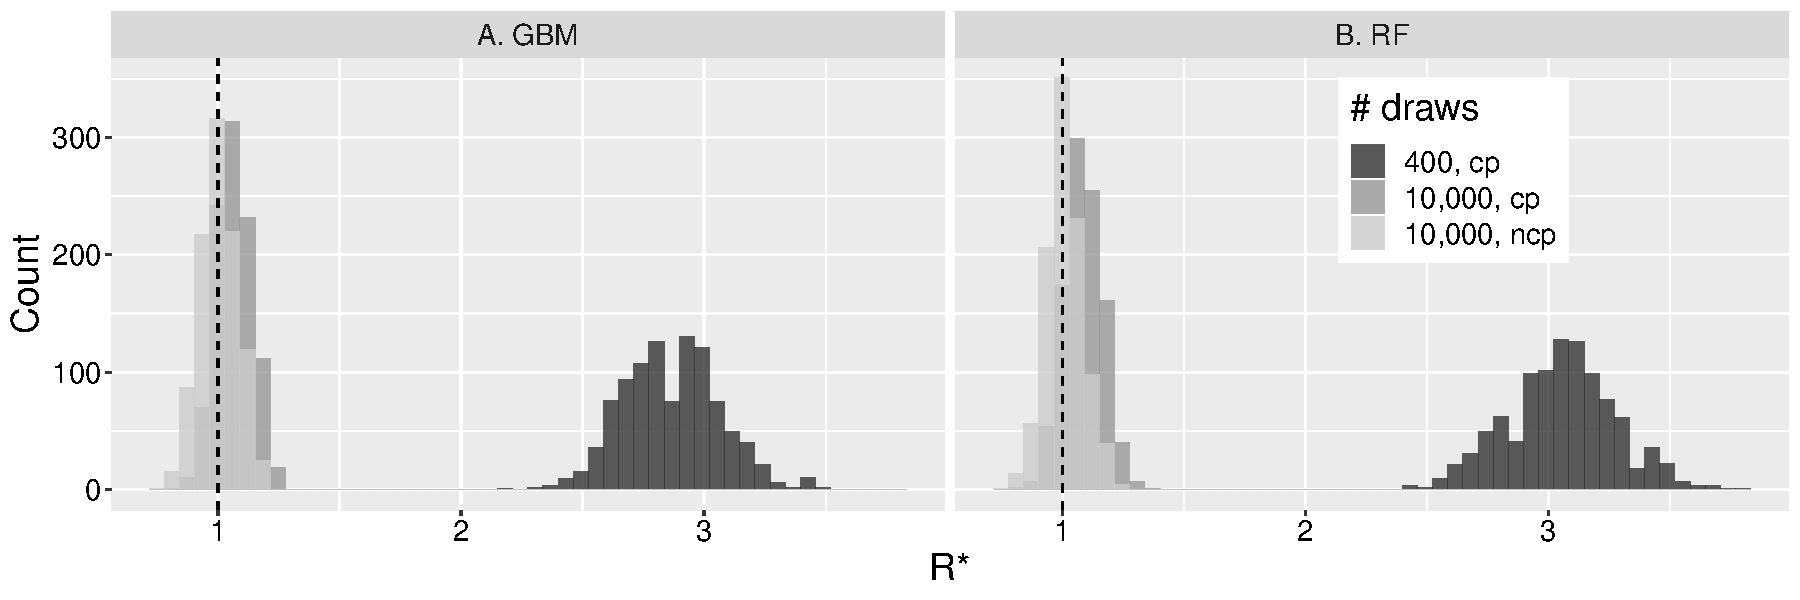
\includegraphics[width=1\textwidth]{mvt_gbm_vs_rf.pdf}}
	\caption{\textbf{Multivariate normal example: GBM (A) versus RF (B) classifiers.} Shows $R^*$ distributions obtained for two MCMC samples (of differing numbers of draws: 400 and 10,000) from the centered parameterisation (``cp'') and one from the non-centered version (``ncp''; with 10,000 draws). Here, we show 1000 $R^*$ draws by Algorithm \ref{alg:R_star_uncertainty} for each MCMC run.}
	\label{fig:mvt_gbm_vs_rf}
\end{figure}

\color{black}

\color{red}
\section{Hierarchical model: Eight schools model supplementary}\label{sec:8_schools_supp}

Fig. \ref{fig:eight_schools_rf} shows the equivalent of Fig. \ref{fig:eight_schools} except using a RF classifier.

\begin{figure}[!htb]
	\centerline{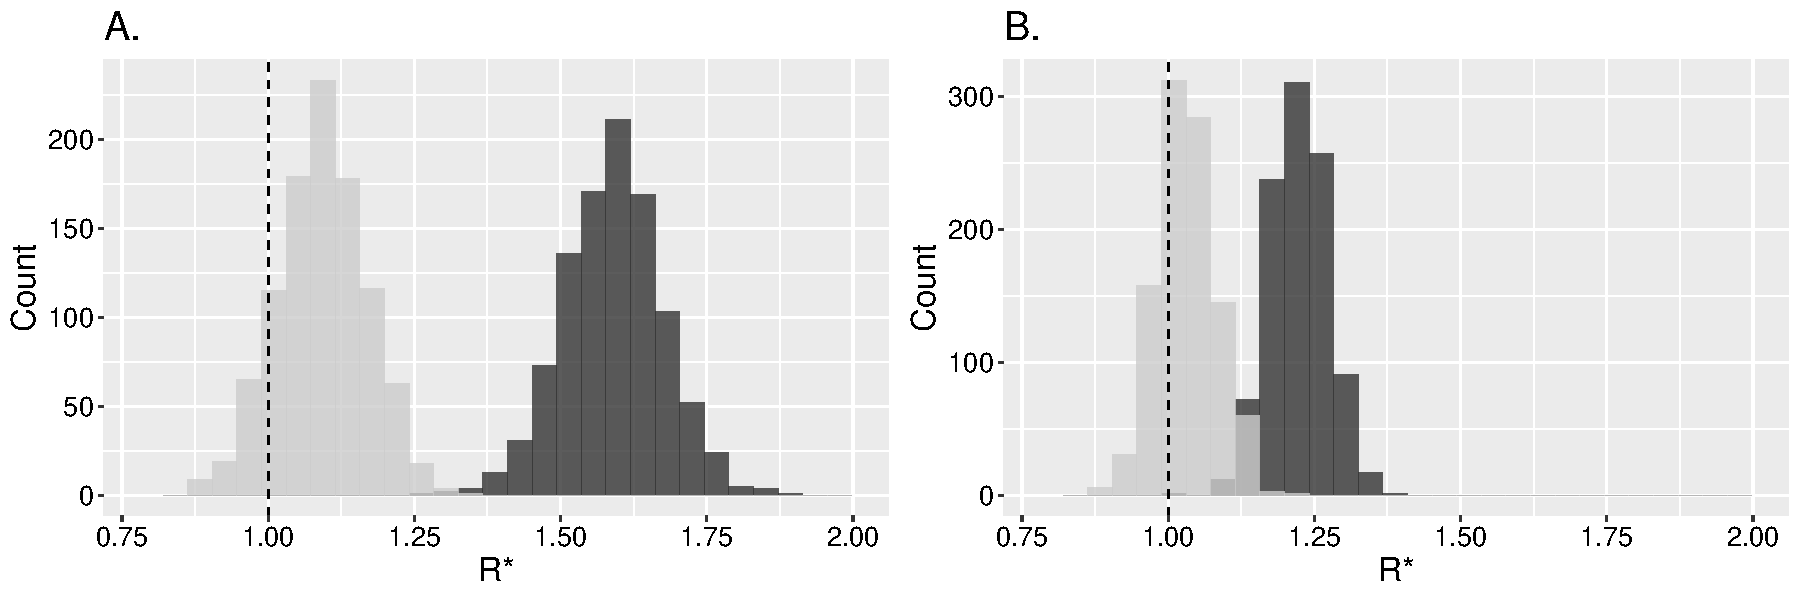
\includegraphics[width=1\textwidth]{eight_schools_rf.pdf}}
	\caption{\textbf{Eight schools example: $R^*$ distributions for a RF classifier.} A shows draws from the $R^*$ distribution when splitting chains in two (resulting in 8 chains); B shows the same but using the 4 original chains. The MCMC samples comprised 2000 draws in all cases, with 1000 used as post-warm-up iterations. In panels A and B, the plots show 1000 $R^*$ draws using Algorithm \ref{alg:R_star_uncertainty} for each parameterisation.}
	\label{fig:eight_schools_rf}
\end{figure}

\color{black}



\section{Wide datasets: multivariate normal}\label{sec:wide}
As the number of parameter dimensions increases, it might be thought that ML algorithms will overfit the data, and, hence, testing set classification would be poor; leading to unreliable determinations of convergence. To test this hypothesis, we investigated two scenarios using a multivariate normal target.

\subsection{250-dimensional model}
In the first of these, we used the 250-dimensional multivariate normal of eq. \eqref{eq:mvt_normal_250} with 250 post-warm-up iterations (after 250 warm-up iterations) for each of 4 chains from Stan's NUTS to calculate $R^*$ distributions as in Algorithm \ref{alg:R_star_uncertainty}. Here, we considered both the centered and non-centered parameterisations, where, in both cases, the number of iterations is comparable to the number of parameters, so the training data is relatively ``wide''. \textcolor{red}{We also calculated $R^*$ distributions using both the GBM and RF classifiers: the $R^*$ distribution in each case is shown in Figs. \ref{fig:mvt_wide_both}A\&B. This figure shows that, across both parameterisations, convergence has not yet been reached since all $R^*$ distributions are shifted rightwards of 1.} The same conclusion is reached if rank-normalised split-$\widehat{R}$ is used instead (Fig. \ref{fig:wide_both_diagnostics}A), since, for both parameterisations, some of the parameters had $\widehat{R}>1.01$. Using bulk- or tail-ESS instead, we conclude that the non-centered parameterisation shows signs of convergence whereas the centered does not (Fig. \ref{fig:wide_both_diagnostics}B\&C). 

\begin{figure}[!htb]
	\centerline{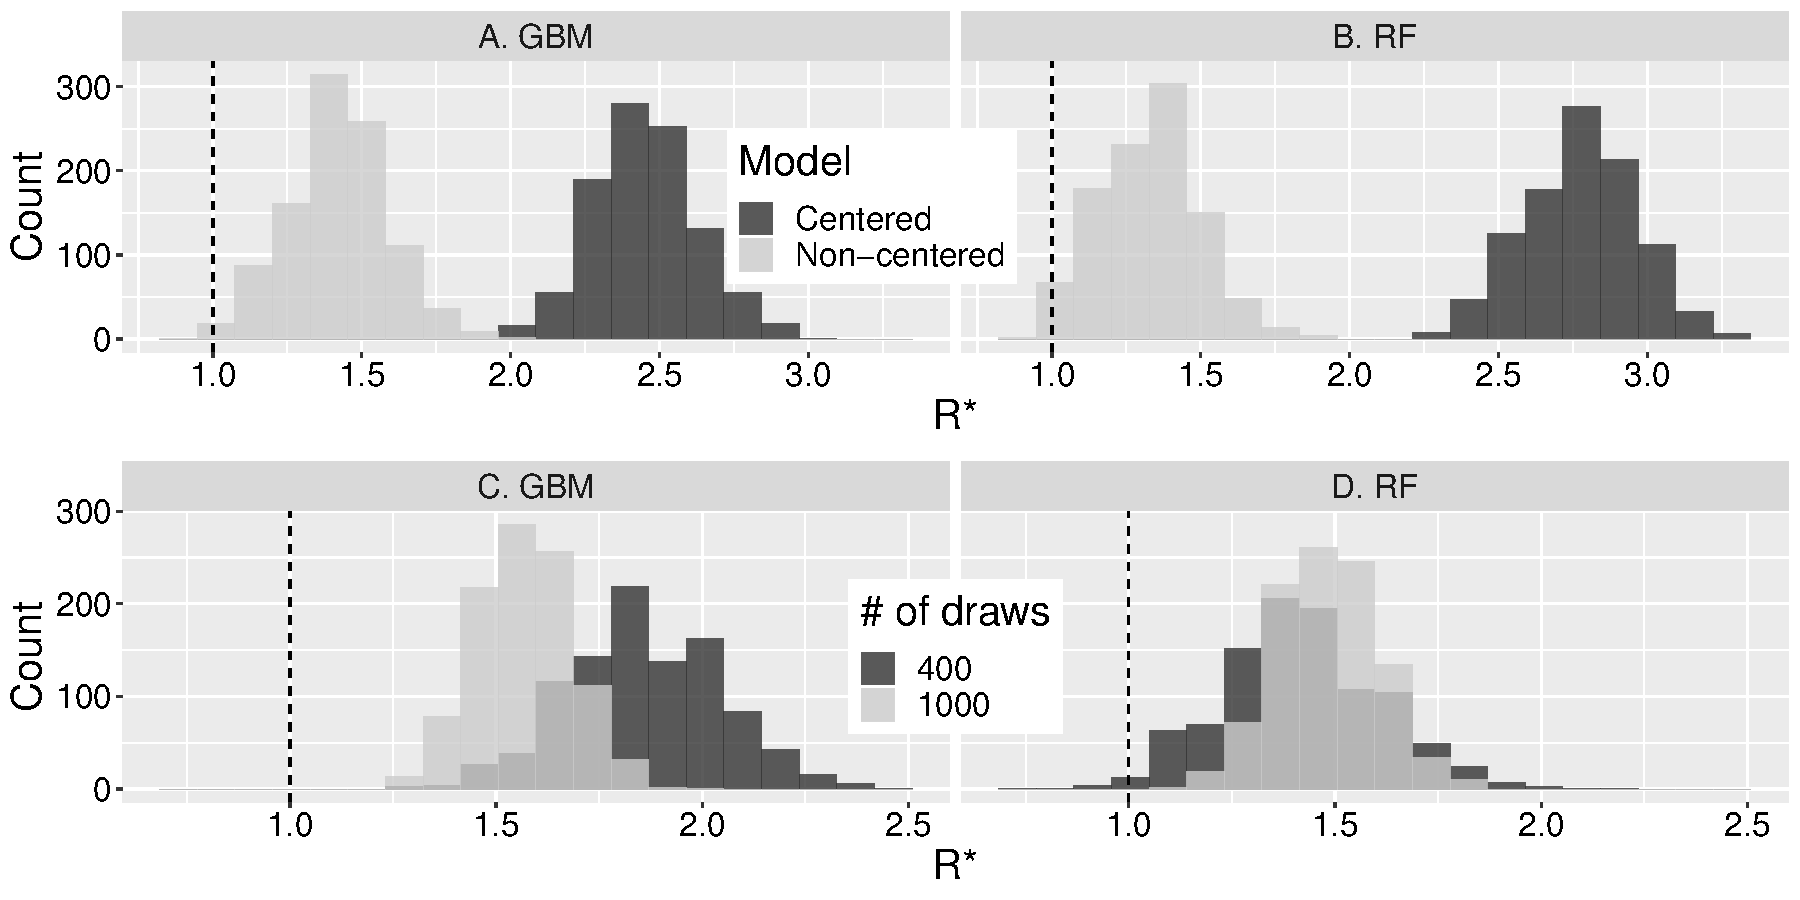
\includegraphics[width=1\textwidth]{mvt_wide_both.pdf}}
	\caption{\textbf{Wide data examples.} Top row shows the $R^*$ distribution for the 250-dimensional example in \S\ref{sec:wide} with 250 post-warm-up iterations per chain from Stan's NUTS algorithm across both model parameterisations; bottom row shows $R^*$ distribution for the 10,000-dimensional example with 400 and 1000 MCMC iterations per chain (although the first half of these were discarded as warm-up). In the left column, results for the GBM classifier are shown; in the right, we show the same for the RF classifier. In all cases, 1000 draws of $R^*$ are plotted as generated by Algorithm \ref{alg:R_star_uncertainty} for a single MCMC run composed of 4 chains.}
	\label{fig:mvt_wide_both}
\end{figure}

\begin{figure}[!htb]
	\centerline{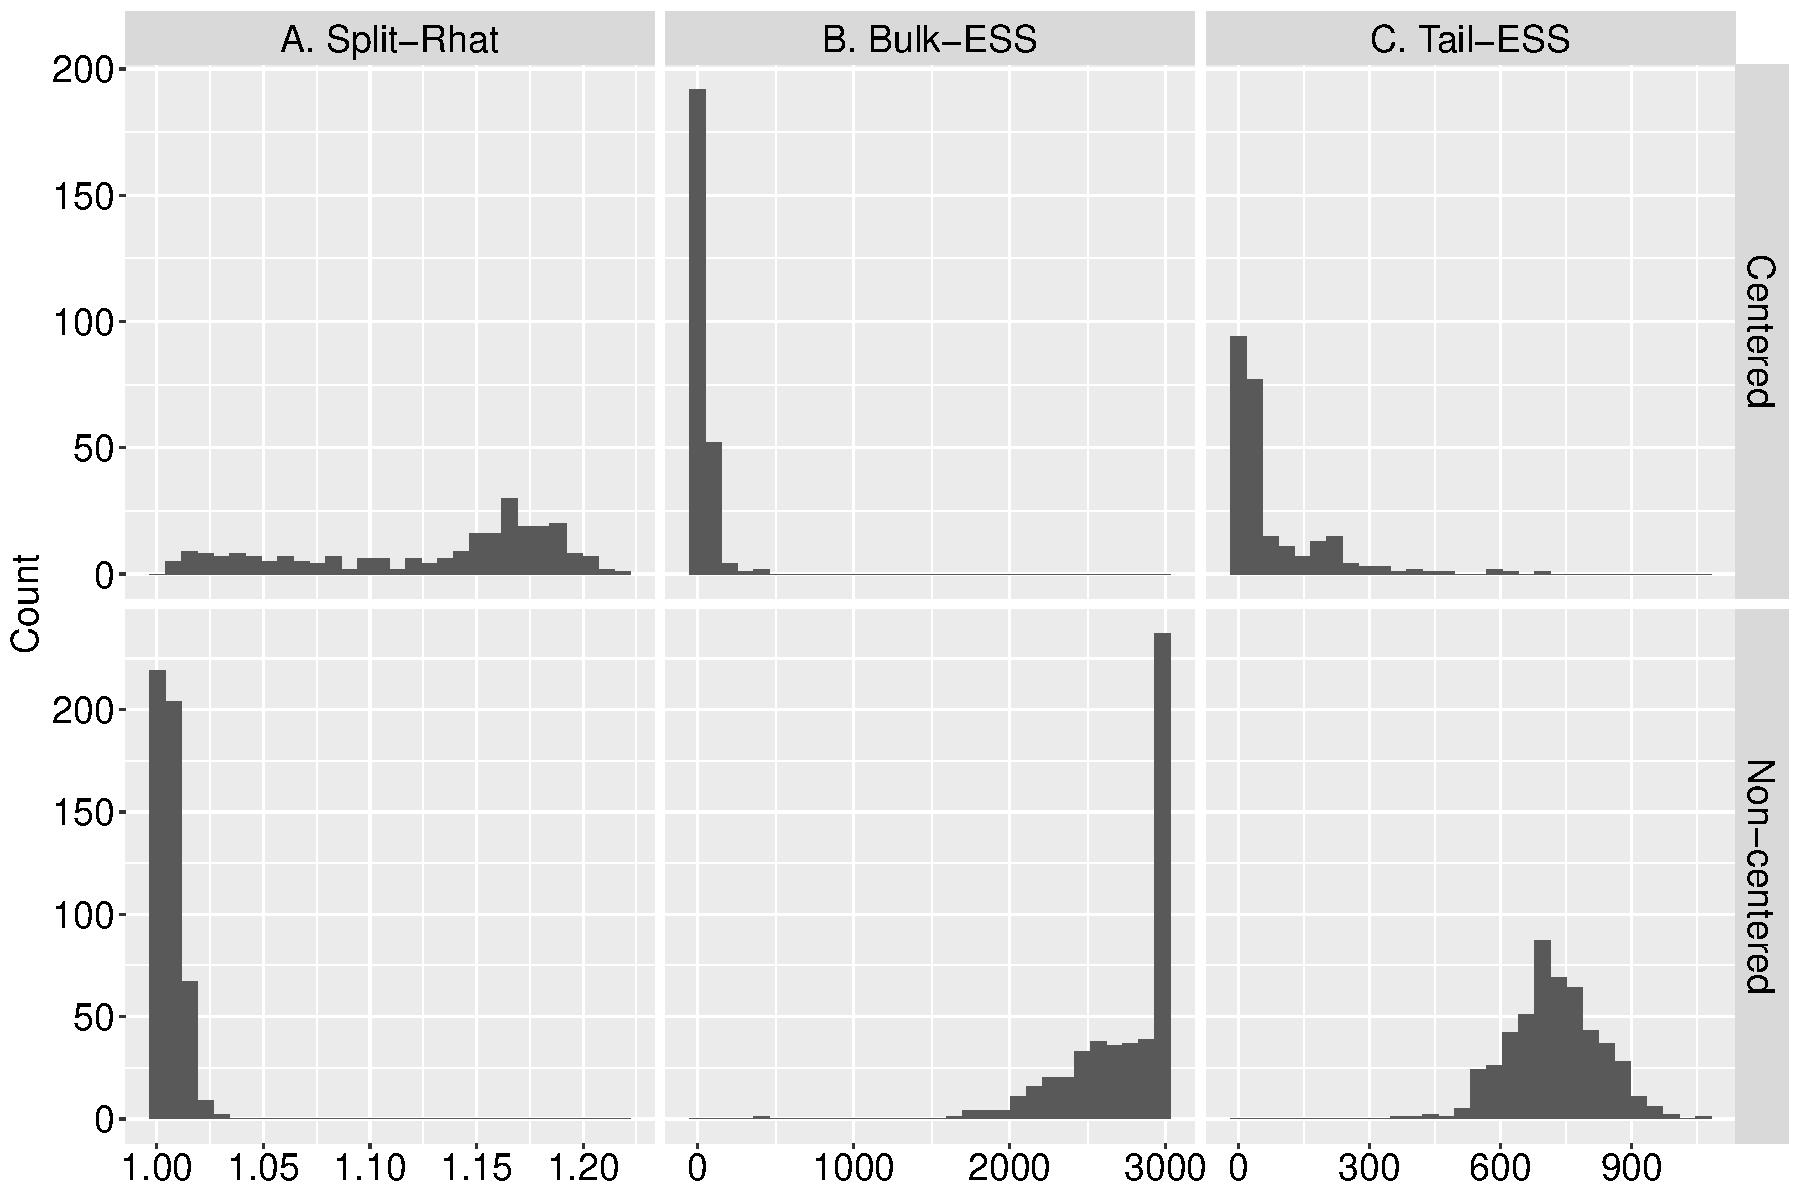
\includegraphics[width=1\textwidth]{wide_both_diagnostics.pdf}}
	\caption{\textbf{Wide data 250-dimensional example: established diagnostics.} The top row shows the results for the centered parameterisation; the bottom row for the non-centered. Column A shows split-$\widehat{R}$; columns B and C show the bulk- and tail-ESS; in each case the statistics are displayed for all model parameters and were calculated using 250 post-warm-up draws from Stan's NUTS algorithm. Note, that it is possible for the ESS to exceed the actual sample size if there is negative autocorrelation in the Markov chains' values. In both cases, the results correspond to a single MCMC run composed of 4 chains.}
	\label{fig:wide_both_diagnostics}
\end{figure}

\subsection{10,000-dimensional model}
We next consider a more challenging example -- a target distribution with 10,000 dimensions. In this case, we assume independent standard normals for each dimension. \textcolor{red}{In Figs. \ref{fig:mvt_wide_both}C\&D, we plot the $R^*$ distributions from GBM and RF classifiers for two MCMC runs targeting this distribution: one with 400 iterations, the other with 1000.} In all cases, the distributions were right of $R^*=1$, indicating non-convergence. These results were also echoed by rank-normalised split-$\widehat{R}$, with \textcolor{red}{19\%} of dimensions having $\widehat{R}>1.01$ for the 400 iteration case and \textcolor{red}{3\%} for the 1000 iteration case.

Overall, the examples in this section suggest that $R^*$ is a conservative measure of convergence: when there are not enough draws, it will tend to diagnose non-convergence. We also note that the statistic took comparable time to calculate relative to existing convergence diagnostics on a desktop computer.

\section{Non-stationary marginals}\label{sec:non-stationary}
If a Markov chain does not mix with itself, this also indicates that convergence has not occurred \citep{gelman2013bayesian}. In this section, we investigate whether $R^*$ can detect non-stationary sampling distributions. \textcolor{red}{In all the examples, we present results for both GBM and RF classifiers.}

\subsection{Trending mean across all chains}\label{sec:non-stationary_chains}
We first recapitulate an example from appendix A in \cite{vehtari2019rank}. This example showed that split-$\widehat{R}$ could detect non-convergence caused by shifts in sampling distributions over time: in their case, they analysed chains with common linear trends in mean. Specifically, they first generated 4 chains by random sampling from a univariate normal distribution, then added a common time trend to each chain, resulting in a univariate distribution whose mean increased during sampling. We first repeat this analysis but using $R^*$ rather than $\widehat{R}$: in Fig. \ref{fig:trends_all_dim}, we show these results. In column A, we show the results for $R^*$ calculated on the 4 chains that ran; column B shows the same calculation but after the chains are split into two equal halves. The rows show the range of sample sizes investigated: 250, 1000 and 4000; the horizontal axis shows the magnitude of time trend added to each sample; for all parameter sets, we run 10 replicates. \textcolor{red}{The points and triangles show $R^*$ derived from GBM and RF classifiers, respectively.} This plot mirrors Fig. 4 in the supplementary materials of \cite{vehtari2019rank} and shows that, without splitting the chains, $R^*$ does not increase with trend whereas, after splitting, it does. As expected, split-$R^*$ is more reliably able to detect non-convergence as sample size increases.

These results make intuitive sense: without systematic between-chain variation, it is not possible to reliably determine which of them caused a particular observation. In this case, because all chains exhibited the same secular trends over time, there would not be differences in their marginals. By splitting chains into two -- the first half being the early phase, and the second half being the later phase with higher mean -- this forces differences in the marginals. This meant it was possible to reliably pick whether an observation was caused by an early phase chain or a later one. As such, we recommend that $R^*$ always be calculated using split chains as is recommended for $\widehat{R}$ \citep{carpenter2017stan,vehtari2019rank}.

\begin{figure}[!htb]
	\centerline{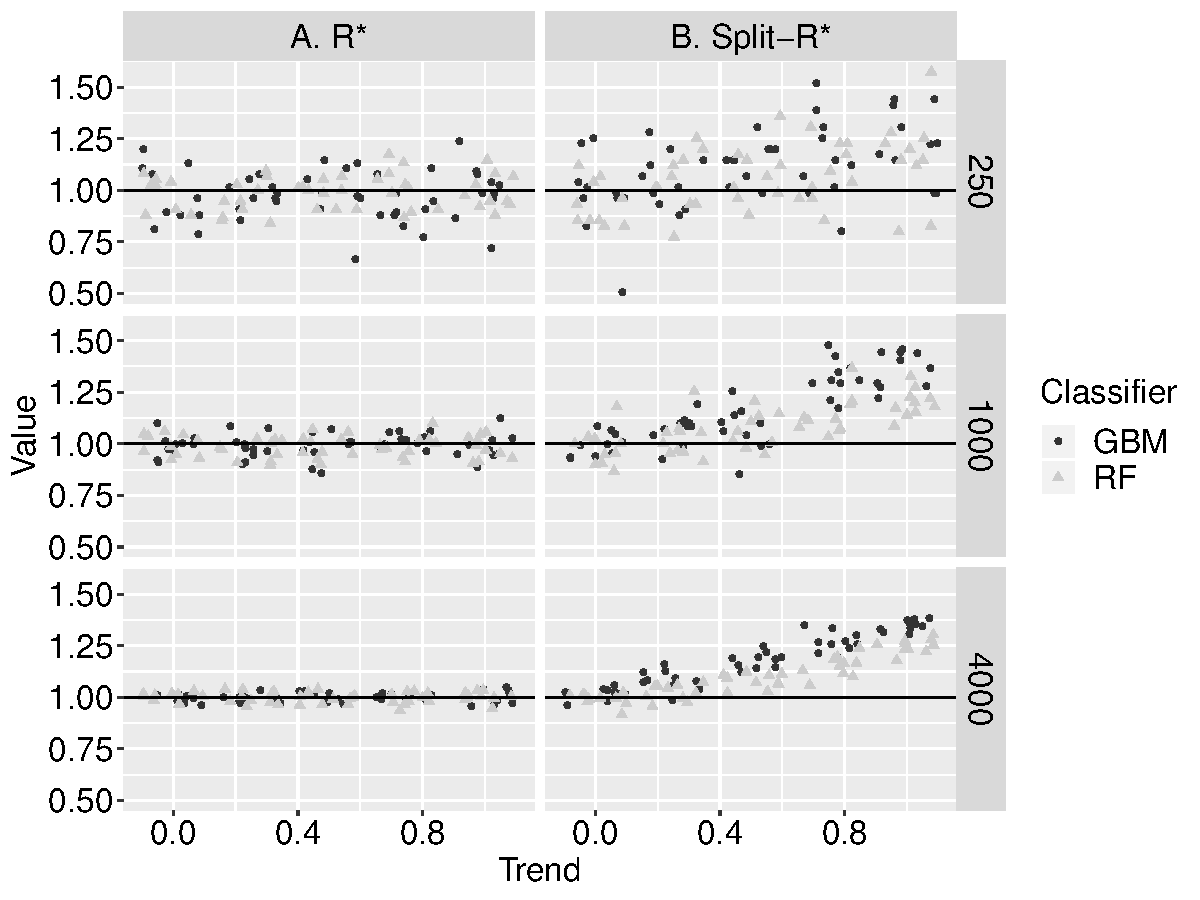
\includegraphics[width=1.0\textwidth]{trends_all_dim.pdf}}
	\caption{\textbf{Univariate trends example.} Points and triangles represent results for the GBM and RF classifiers, respectively. Column A represents results for $R^*$ calculated using Algorithm \ref{alg:R_star} on the 4 chains; column B  shows the same calculation after each chain is split into two halves. The rows present the differing sample sizes. The horizontal axis measures (half) the change in mean across the whole sample: so a value ``1'' indicates the mean increases by 2 units from the start to end of sampling. At each parameter set, 10 replicates were run and jitter was added to the points.}
	\label{fig:trends_all_dim}
\end{figure}

\subsection{Trending mean in a single dimension}\label{sec:non-stationary_single}
We next consider whether split-$R^*$ can detect non-convergence when only a single dimension trends. In Fig. \ref{fig:trends_one_dim}, we show how $R^*$ performs across a range of target dimensions. In the simulations here, all dimensions bar one are stationary; the remaining dimension has a linear trend added to it. In all cases, \textcolor{red}{across both GBM and RF classifiers}, split-$R^*$ increased with trend. Indeed, differences in the typical values of this metric were not apparent across the different target dimensions considered. This suggests split-$R^*$ can robustly determine chain identity if only a single dimension has a non-stationary sampling distribution.


\begin{figure}[!htb]
	\centerline{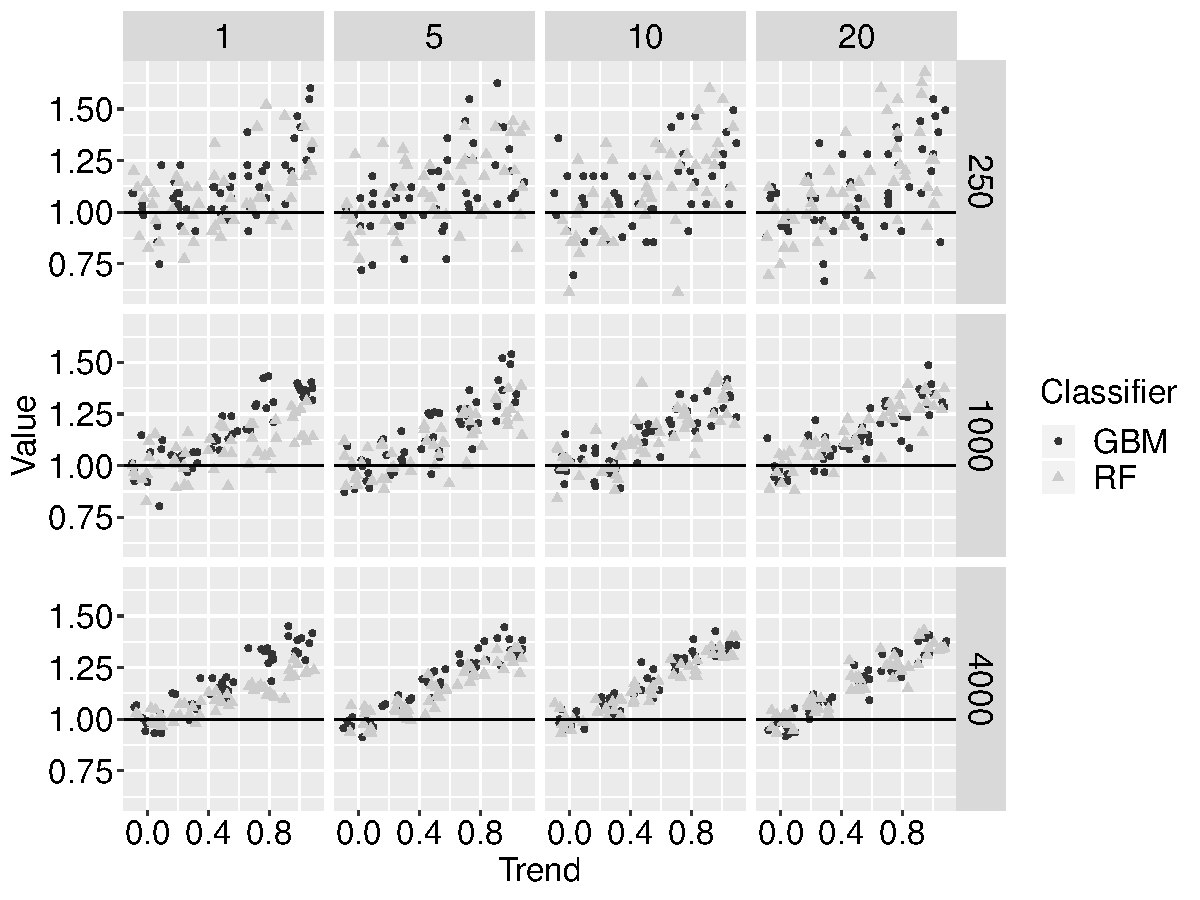
\includegraphics[width=1.0\textwidth]{trends_one_dim.pdf}}
	\caption{\textbf{Multivariate trends example with split-$R^*$.} Points and triangles represent results for the GBM and RF classifiers, respectively. The columns present different dimensionalities of the target distribution; the rows present different sample sizes. The horizontal axis measures (half) the change in mean across the single dimension that had a trend added to it: a value ``1'' indicates its mean increases by 2 units from the start to end of sampling; all other dimensions (if dimensions exceeded 1) had stationary distributions. At each parameter set, 10 replicates were run and jitter was added to the points.}
	\label{fig:trends_one_dim}
\end{figure}

\subsection{Trending covariance}\label{sec:non-stationary_covariance}
Means that trend over time is one form of non-stationarity; another is a time-varying covariance. Next, we consider a bivariate normal with (constant) standard normal marginals but where the correlation between dimensions trends over time. Specifically, we allow the correlation to increase linearly from $-\rho$ and $\rho$ throughout the course of simulations and use i.i.d. draws from the process across 4 ``chains''. Again, as before, $R^*$ calculated on unsplit chains is unable to detect this form of non-stationarity, since there are no inter-chain differences in the sampling distribution. Similarly, split-$\widehat{R}$ does not detect this form of non-convergence since the marginal distribution across chains does not vary over time (Fig. \ref{fig:trends_joint_distribution}A). By contrast, split-$R^*$ can (Fig. \ref{fig:trends_joint_distribution}B), since it uses all information in the samples, including the covariance structure.

\begin{figure}[!htb]
	\centerline{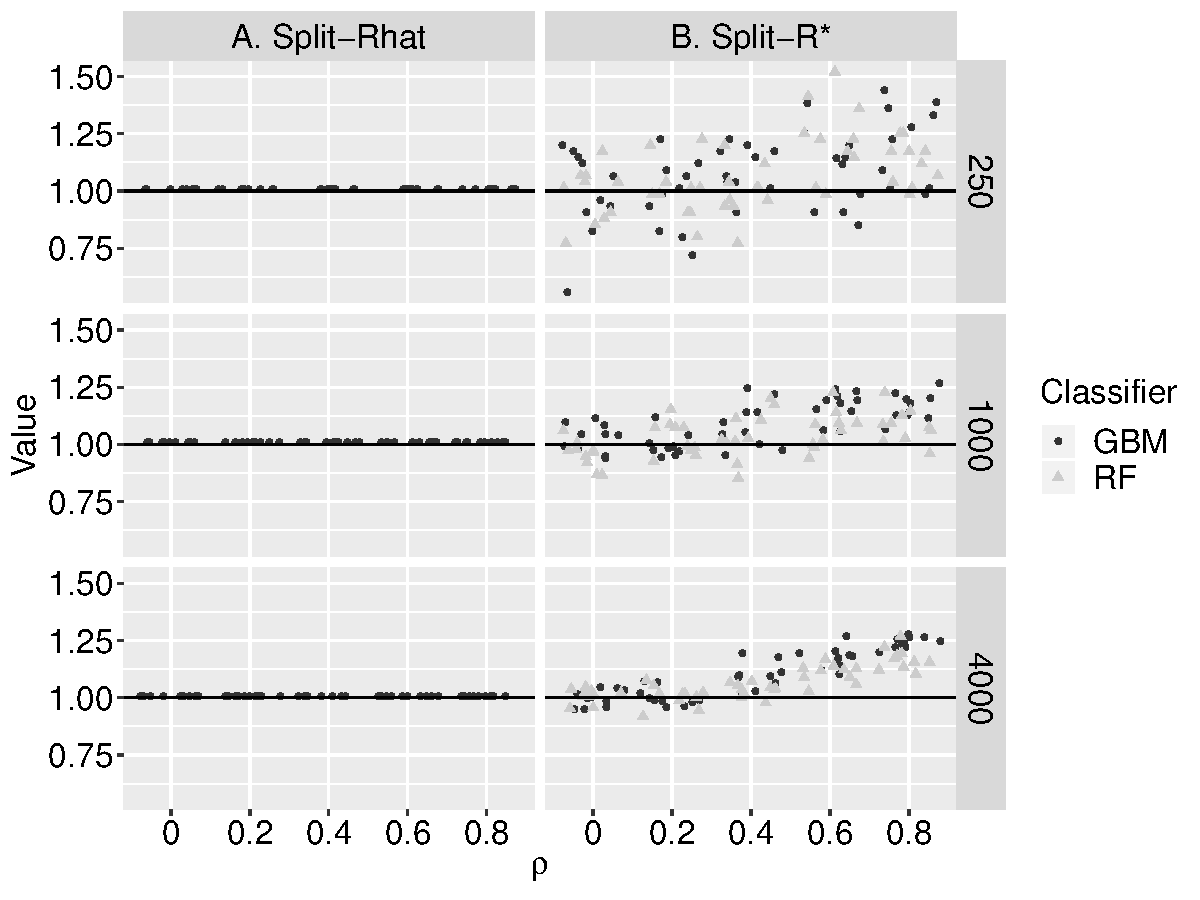
\includegraphics[width=1.0\textwidth]{trends_joint_distribution.pdf}}
	\caption{\textbf{Bivariate normal with trending correlation example.} Points and triangles represent results for the GBM and RF classifiers, respectively. Column A shows the results for split-$\widehat{R}$; column B for $R^*$; the rows present the differing sample sizes. The horizontal axis measures (half) the change in correlation across the whole sample: so a value ``0.5'' indicates the correlation increases by 1 unit (from -0.5 to 0.5) from the start to end of sampling. At each parameter set, 10 replicates were run and jitter was added to the points.}
	\label{fig:trends_joint_distribution}
\end{figure}

\subsection{Chain persistence}\label{sec:non-stationary_persistence}
When forming training and testing sets as part of the ML algorithm used to determine $R^*$, the testing set is effectively treated as a sort of ``independent'' hold-out dataset. Markov chains, in general, have persistence, meaning that the test set will not be truly independent and can -- according to the level of autocorrelation in the chains -- be highly related to the training set. In this section, we investigate how this autocorrelation affects the performance of $R^*$. The difficulty with this question is that higher chain autocorrelation typically means the sampling distribution is a rougher approximation of the target, so $R^*$ should be higher due to the properties of the sampling distribution. It could also be higher because the training set is less distinct from the testing set.

To investigate this, we generated AR(1) processes (as defined in eq. (\ref{eq:ar1})) with autocorrelations, $\rho$, ranging from 0.8-1 and, in each case, calculated $R^*$ via Algorithm \ref{alg:R_star}. Note, that only when $|\rho|<1$ is the marginal distribution defined by this process itself stationary; at $\rho=1$, its variance increases linearly with time, so, by definition, is not converged. In Fig. \ref{fig:trends_ar1}, we show the results of these simulations across various numbers of iterations: 250, 1000 and 4000 (different panels). In all cases, $R^*>1$ whenever $\rho=1$, indicating lack of convergence. As $\rho$ declined, so did $R^*$.

Notably, as the number of iterations increased, the values of $R^*$ for $\rho<1$ declined, whereas $R^*$ for $\rho=1$ actually increased: this is most easily seen by examining Fig. \ref{fig:trends_ar1_transposed} (which shows the same data as in Fig. \ref{fig:trends_ar1} but in a different way). This characteristic is exactly as desired: larger sample sizes should yield a sampling distribution closer to convergence for $\rho<1$; the same for $\rho=1$ produces distributions that are no closer to convergence, and more samples allows better determination of this non-convergence.

Overall, it seems that $R^*$ is a conservative measure and with greater chain autocorrelation it suggests more draws are necessary for convergence.

\begin{figure}[!htb]
	\centerline{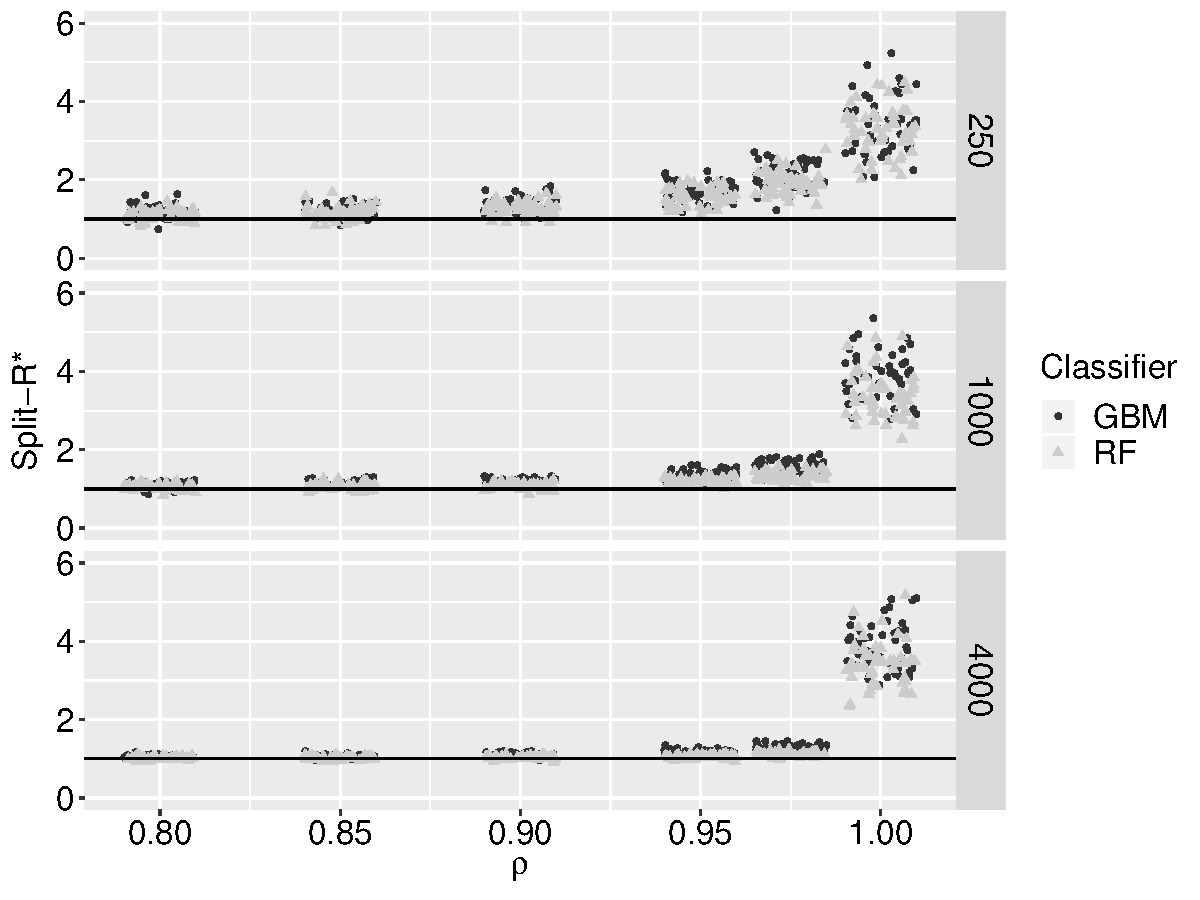
\includegraphics[width=1.0\textwidth]{trends_ar1.pdf}}
	\caption{\textbf{Non-stationary distribution: AR(1) example.} Points and triangles represent results for the GBM and RF classifiers, respectively. The horizontal axis measures the autocorrelation of the AR(1) processes; the vertical axis shows the value of $R^*$ calculated on chains split in half; each panel shows a different number of iterations. At each parameter set, 10 replicates were run and jitter was added to the points. The black line shows $R^*=1$.}
	\label{fig:trends_ar1}
\end{figure}

\begin{figure}[!htb]
	\centerline{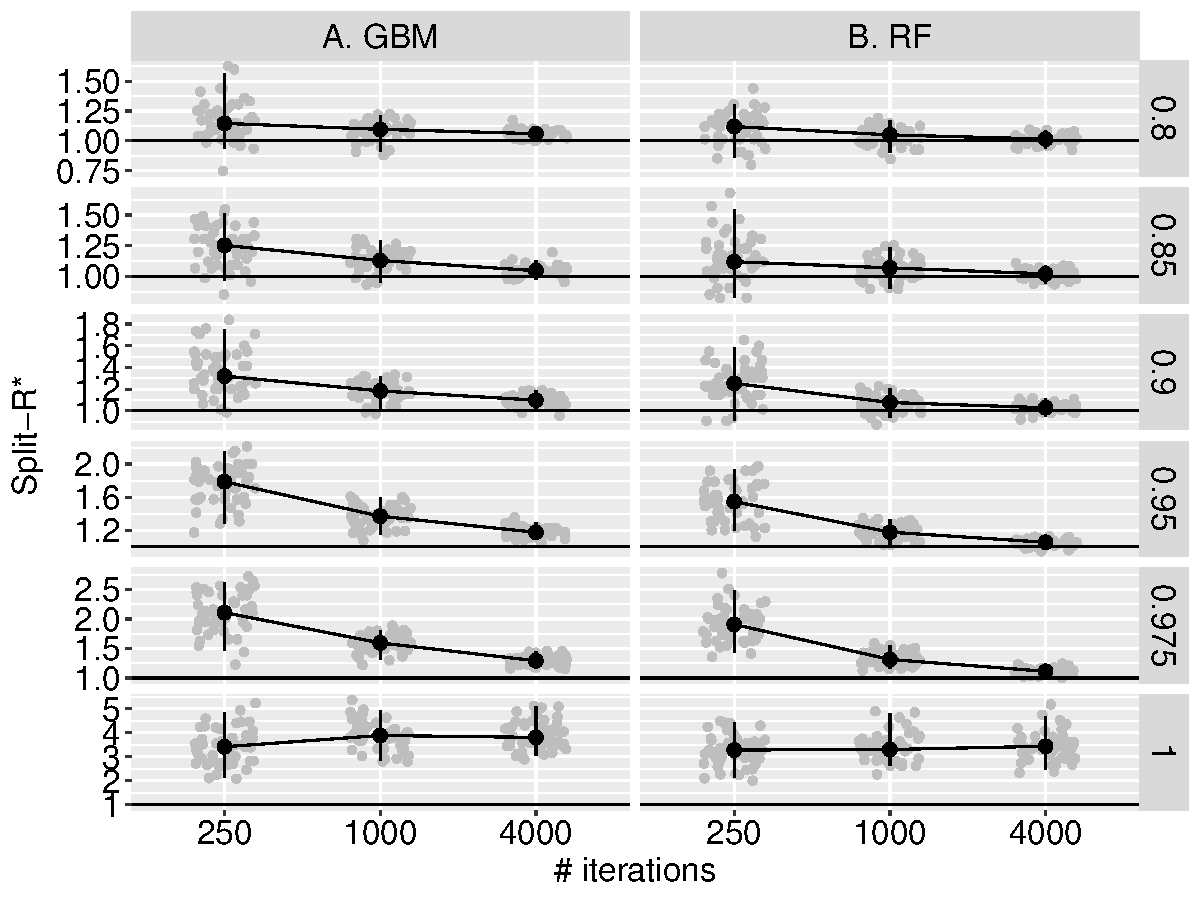
\includegraphics[width=1.0\textwidth]{trends_ar1_transposed.pdf}}
	\caption{\textbf{Non-stationary distribution: AR(1) example alternative view.} Column A shows the results for a GBM classifier; column B for a RF classifier. The horizontal axis measures the number of iterations; the vertical axis shows the value of $R^*$ calculated on chains split in half; each panel shows a different value of autocorrelation. At each parameter set, 10 replicates were run and jitter was added to the points. The black dots show the median $R^*$ values at each parameter set; upper and lower whiskers show 2.5\% and 97.5\% quantiles. The black horizontal line shows $R^*=1$. }
	\label{fig:trends_ar1_transposed}
\end{figure}

\section{Many parameter models: ovarian and prostate analysis}\label{sec:prostate}
In this section, we analyse two Bayesian models both fit to real data. \textcolor{red}{In both examples, we illustrate $R^*$ distributions derived only from GBM classifiers.} The first is a logistic regression model fit to microarray ovarian cancer data with 54 data points and 1536 predictor variables; overall, this model has 4719 parameters. Since there are relatively few data points relative to the number of predictors, regularised horseshoe priors are specified on the regression coefficients \citep{piironen2017sparsity} since most are expected to be zero. This dataset has been used for benchmarking in the past (see, for example, \cite{schummer1999comparative,hernandez2010expectation,paananen2019implicitly}) and is known to result in a multimodal posterior.

The other dataset we use is of similar form but for prostate cancer. The original form of the dataset is described here: \cite{singh2002gene}. We use a filtered version of the dataset as detailed here: \cite{yang2006stable}, which we also analysed using logistic regression with regularised horseshoe priors. It has 18,105 parameters in total. 

For each model, we consider two MCMC runs: one with 4 chains run with 800 thinned post-warm-up iterations (9000 total iterations with 1000 discarded as warm-up; 8000 post-warm-up iterations thinned by a factor of 10); another with 16 chains run with 1000 post-warm-up iterations each (500 warm-up iterations discarded and no thinning).

For the ovarian model, we show the results in Fig. \ref{fig:ovarian}. In Fig. \ref{fig:ovarian}A, we show the $R^*$ distributions for each model run, which show that, whereas the ``long'' model run has converged, the ``short'' one has yet to do so. Whilst it is harder to discern, this pattern is mirrored in Fig. \ref{fig:ovarian}B, since the long model has $\widehat{R}<1.01$ for all parameters, whereas the short model had \textcolor{red}{83} parameters where this was not the case. Similarly, in Figs. \ref{fig:ovarian}C and \ref{fig:ovarian}D, which show the bulk-ESS and tail-ESS respectively, it is evident that, for the short model, there remain a few parameters with low effective sample sizes, whereas the long model has more consistent values for this metric.

\begin{figure}[!htb]
	\centerline{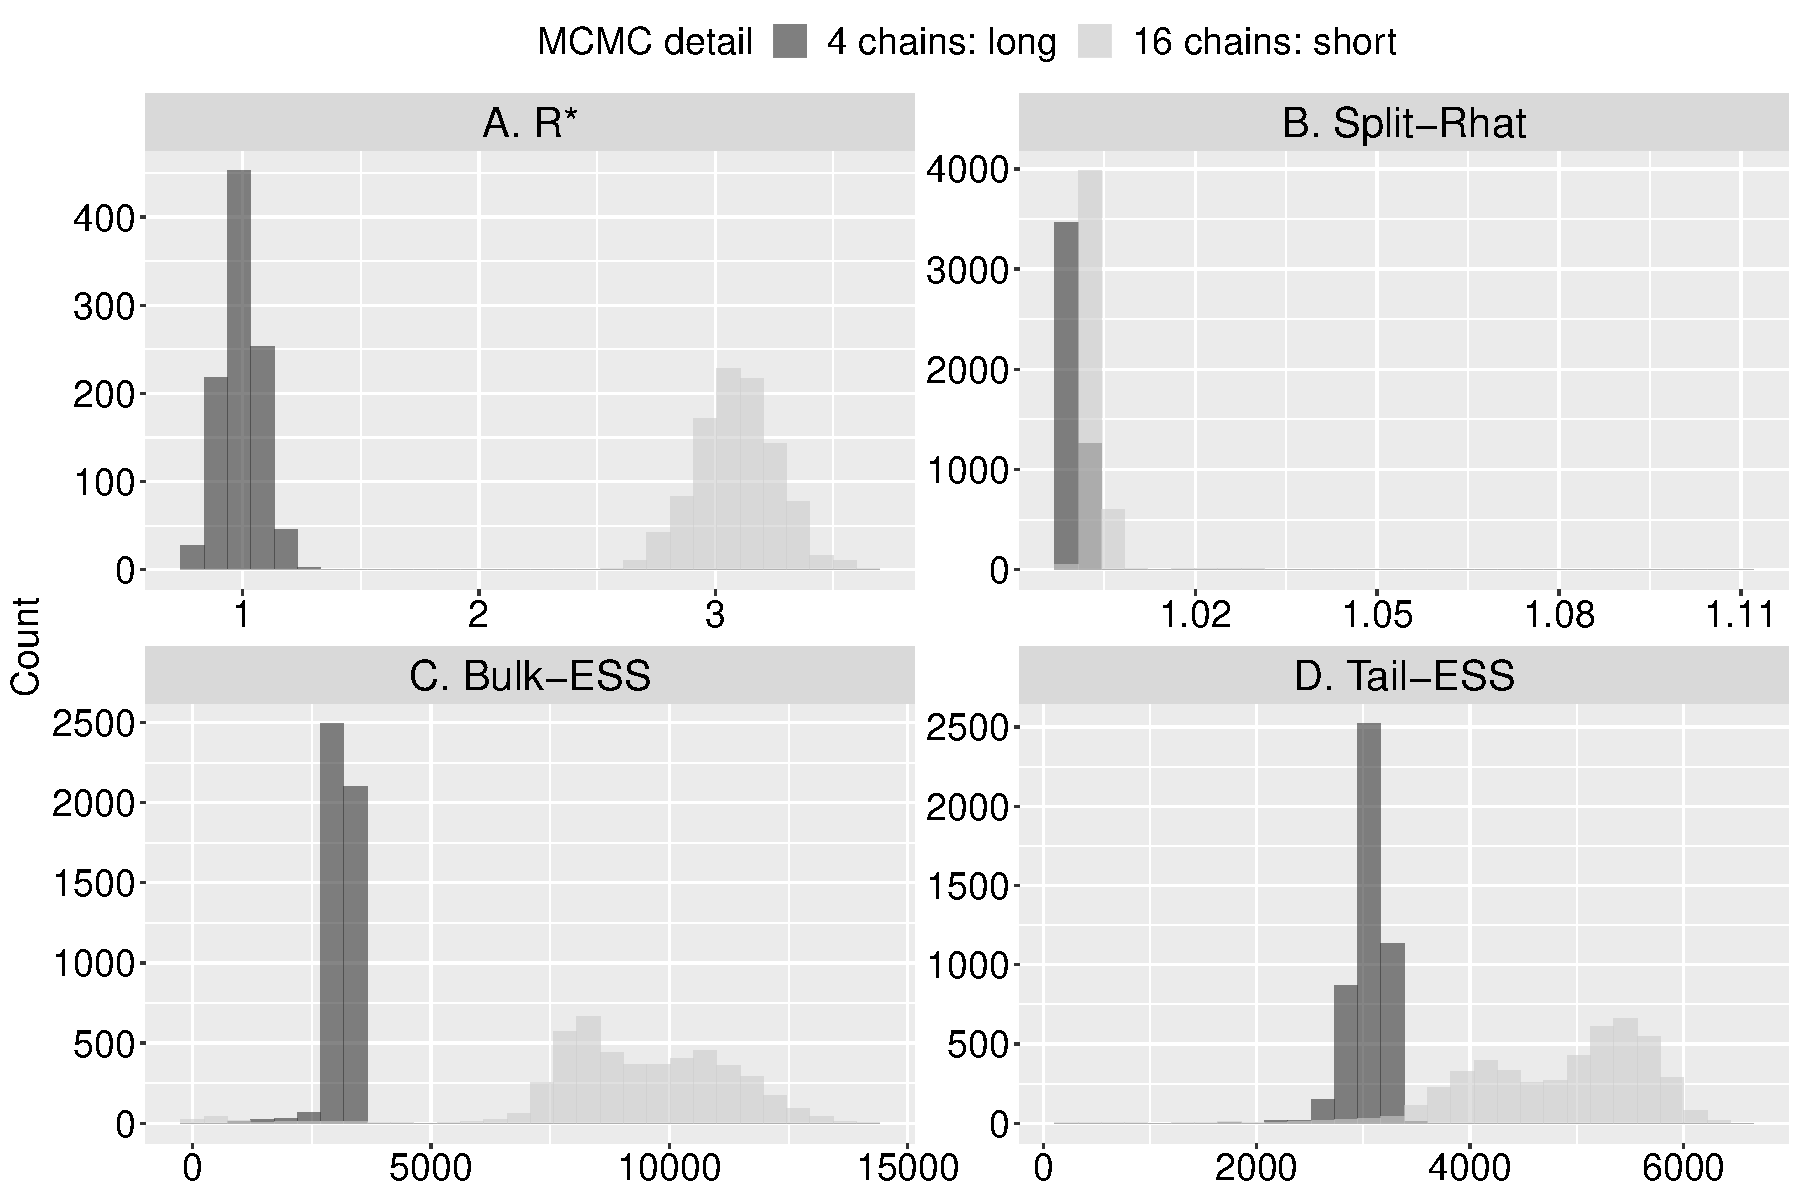
\includegraphics[width=1.0\textwidth]{ovarian.pdf}}
	\caption{\textbf{Ovarian example.} In all plots, we show the results from two model runs: one with 4 chains run with 800 thinned post-warm-up iterations (9000 total iterations with 1000 discarded as warm-up; 8000 post-warm-up iterations thinned by a factor of 10); another with 16 chains run with 1000 post-warm-up iterations each (500 warm-up iterations discarded and no thinning). In A, $R^*$ distributions (with 1000 draws each using Algorithm \ref{alg:R_star_uncertainty}) using the GBM classifier are shown; B shows rank-normalised split-$\widehat{R}$ values across all parameters; C shows bulk-ESS across all parameters; and D shows tail-ESS across parameters.}
	\label{fig:ovarian}
\end{figure}

For the prostate model, we show the results in Fig. \ref{fig:prostate}. Since this model has nearly four times as many parameters as the ovarian model, it was more computationally expensive to estimate $R^*$ for it. To handle this, we thinned down the parameters by a factor of 5 for the long model, recognising that, of course, this measure will make it more likely that we diagnose convergence. Despite this, both $R^*$ measures indicated that the MCMC runs had yet to converge (Fig. \ref{fig:prostate}A), which was mirrored by the other metrics considered (Figs. \ref{fig:prostate}B,C\&D).

\begin{figure}[!htb]
	\centerline{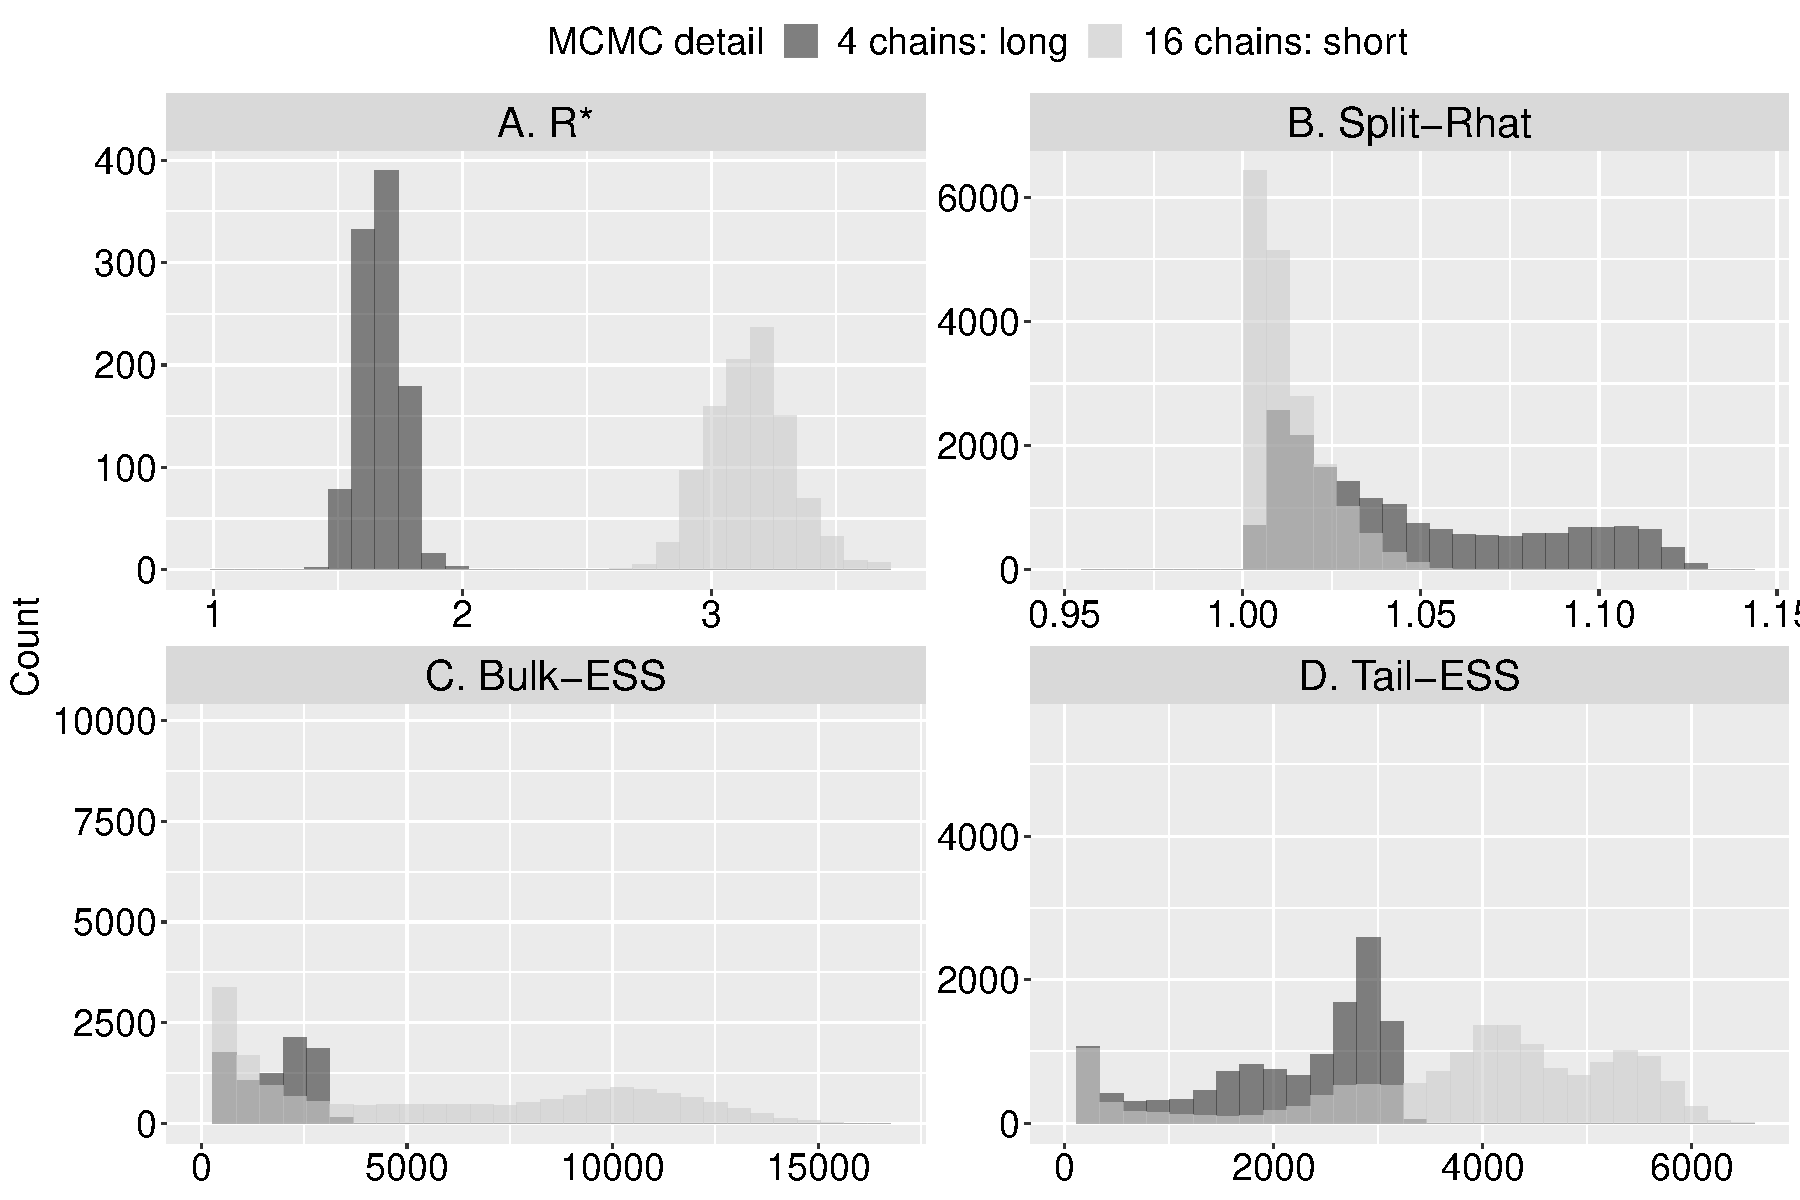
\includegraphics[width=1.0\textwidth]{prostate.pdf}}
	\caption{\textbf{Prostate example.} In all plots, we show the results from two model runs: one with 4 chains run with 800 thinned post-warm-up iterations (9000 total iterations with 1000 discarded as warm-up; 8000 post-warm-up iterations thinned by a factor of 10); another with 16 chains run with 1000 post-warm-up iterations each (500 warm-up iterations discarded and no thinning). In A, $R^*$ distributions (with 1000 draws each using Algorithm \ref{alg:R_star_uncertainty}) using the GBM classifier are shown -- for the long run, these were calculated after thinning the parameters by a factor of 5; B shows rank-normalised split-$\widehat{R}$ values across all parameters; C shows bulk-ESS across all parameters; and D shows tail-ESS across parameters.}
	\label{fig:prostate}
\end{figure}

\color{red}
\section{Discrete distributions}\label{sec:discrete}
In this section, we compare the performance of $R^*$ and $\widehat{R}$ on a univariate discrete target distribution. To do so, we generate draws from four discrete Markov chains, following a 1st order Markov process with transition probabilities,
%
\begin{equation}
p_{ij} = \text{Pr}(X_{n+1}=j|X_n=i),
\end{equation}
%
where $p_{ij}$ is the probability of transitioning from state $i$ at time $n$ to state $j$ at time $n+1$, and $X(0)=1$. The target distribution is, hence, the stationary distribution of this process.

\subsection{Small state-space}\label{sec:discrete_small}
We first consider a univariate discrete distribution with four states. In three of the four chains, we generate draws using a transition probability matrix:
%
\begin{gather}
\boldsymbol{P}
=
\begin{bmatrix}
0 & 1/2 & 1/2 & 0\\
1/2 & 0 & 1/3 & 1/6\\
1/4 & 1/4 & 1/4 & 1/4\\
0 & 1 & 0 & 0
\end{bmatrix},
\end{gather}
%
which implies a stationary target distribution with the following probability simplex $\pi_1 = (11/46, 15/46, 14/46, 6/46)$.

For the fourth chain, we specify differing transition probability matrices in each of three sets of results. In the first, we assume $\boldsymbol{P}_1=\boldsymbol{P}$ (i.e. the same as used for the other three chains); in the second and third cases, we assume this transition matrix is given by:
%
\begin{gather}
\boldsymbol{P}_2
=
\begin{bmatrix}
0 & 1/2 & 1/2 & 0\\
1/2 & 0 & 1/3 & 1/6\\
5/8 & 1/8 & 1/8 & 1/8\\
1/2 & 1/2 & 0 & 0
\end{bmatrix},\quad
\boldsymbol{P}_3
=
\begin{bmatrix}
0 & 1/2 & 1/2 & 0\\
1/2 & 0 & 1/3 & 1/6\\
1 & 0 & 0 & 0\\
1 & 0 & 0 & 0
\end{bmatrix}.
\end{gather}
%
These correspond to stationary probability simplices:
%
\begin{equation}
\pi_2 = (71/198, 17/66, 10/33, 8/99), \quad \pi_3 = (4/9, 2/9, 8/27, 1/27).
\end{equation}
%
The three stationary distributions corresponding to each transition probability matrix are shown in Fig. \ref{fig:discrete_stationary}. This illustrates that there is an ordering among the stationary distributions $\pi_1\sim\pi_2\sim\pi_3$, meaning $\pi_1$ is most similar to $\pi_2$, and $\pi_3$ is most similar to $\pi_2$. Put another way, $\pi_3$ is most different from $\pi_1$.

\begin{figure}[!htb]
	\centerline{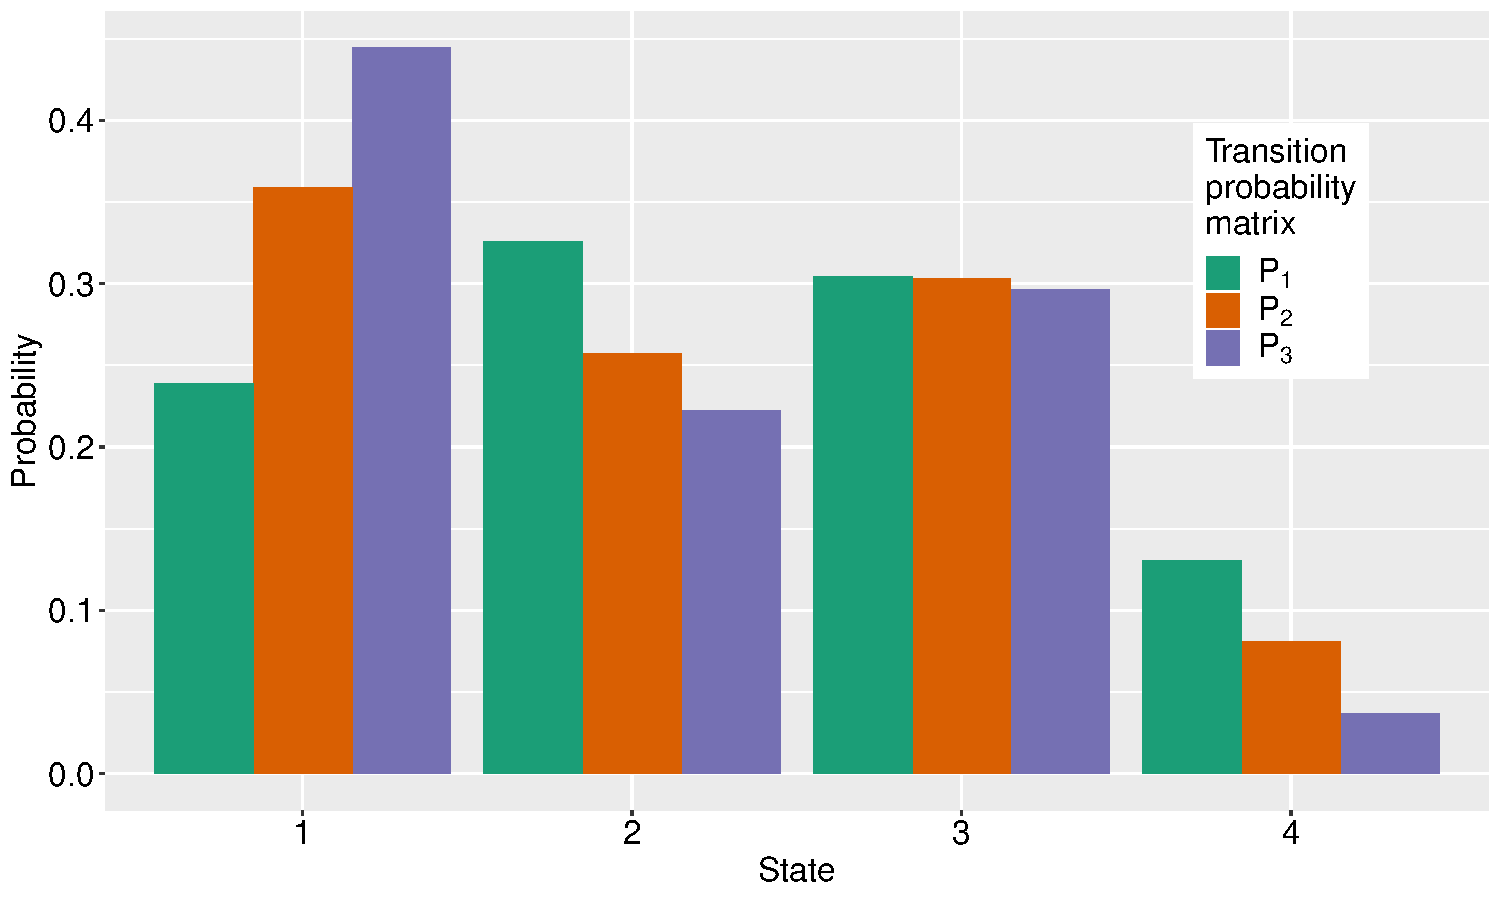
\includegraphics[width=1.0\textwidth]{discrete_stationary.pdf}}
	\caption{\textbf{Discrete distribution example: stationary distributions.} The three colours illustrate the stationary distributions of the Markov chains corresponding to the matrices $P_1$, $P_2$ and $P_3$ defined in \S\ref{sec:discrete}.}
	\label{fig:discrete_stationary}
\end{figure}

For each of these three cases, we consider a range of sample sizes across each of the four chains: 1000, 2000, 5000 and 10,000. At each combination of transition probability matrix (for the fourth chain) and sample size, we perform 40 replicates. In each replicate, we calculate both $R^*$ using a GBM classifier and rank-normalised split-$\widehat{R}$. The results of these experiments are shown in Fig. \ref{fig:discrete}. In the horizontal axes of both panels, we show the sample size. The vertical axis indicates the value of $R^*$ and split-$\widehat{R}$ in panels A and B, respectively. The stacked sub-panels within A and B indicate the transition matrix used for the fourth chain. Since $\boldsymbol{P}_1=\boldsymbol{P}$, the stationary distribution for the other three chains, both diagnostics should tend towards indicating convergence in these cases, and, for both statistics, this was typically the case. For $R^*$, the replicates were centred on $R^*=1$, although the stochasticity of replicates meant that, in some cases, $R^*>1$. Whereas, $\widehat{R}$ was similarly close to 1 in all cases. Considering the simulations using $\boldsymbol{P}_2$ for the fourth chain transition probability matrix, $R^*>1$ across a majority of replicates, and this majority increased with sample size. In this case, $1.01>\widehat{R}>1$ for all replicates across the various sample sizes. For simulations using $\boldsymbol{P}_3$ for the fourth chain transition probability matrix, $R^*>1$ across all replicates and the magnitude of median $R^*$ increased with sample size; in this case, $\widehat{R}>1.01$ in all replicates.

This example shows that $R^*$ can detect poor convergence for discrete parameter spaces, like $\widehat{R}$.


\begin{figure}[!htb]
	\centerline{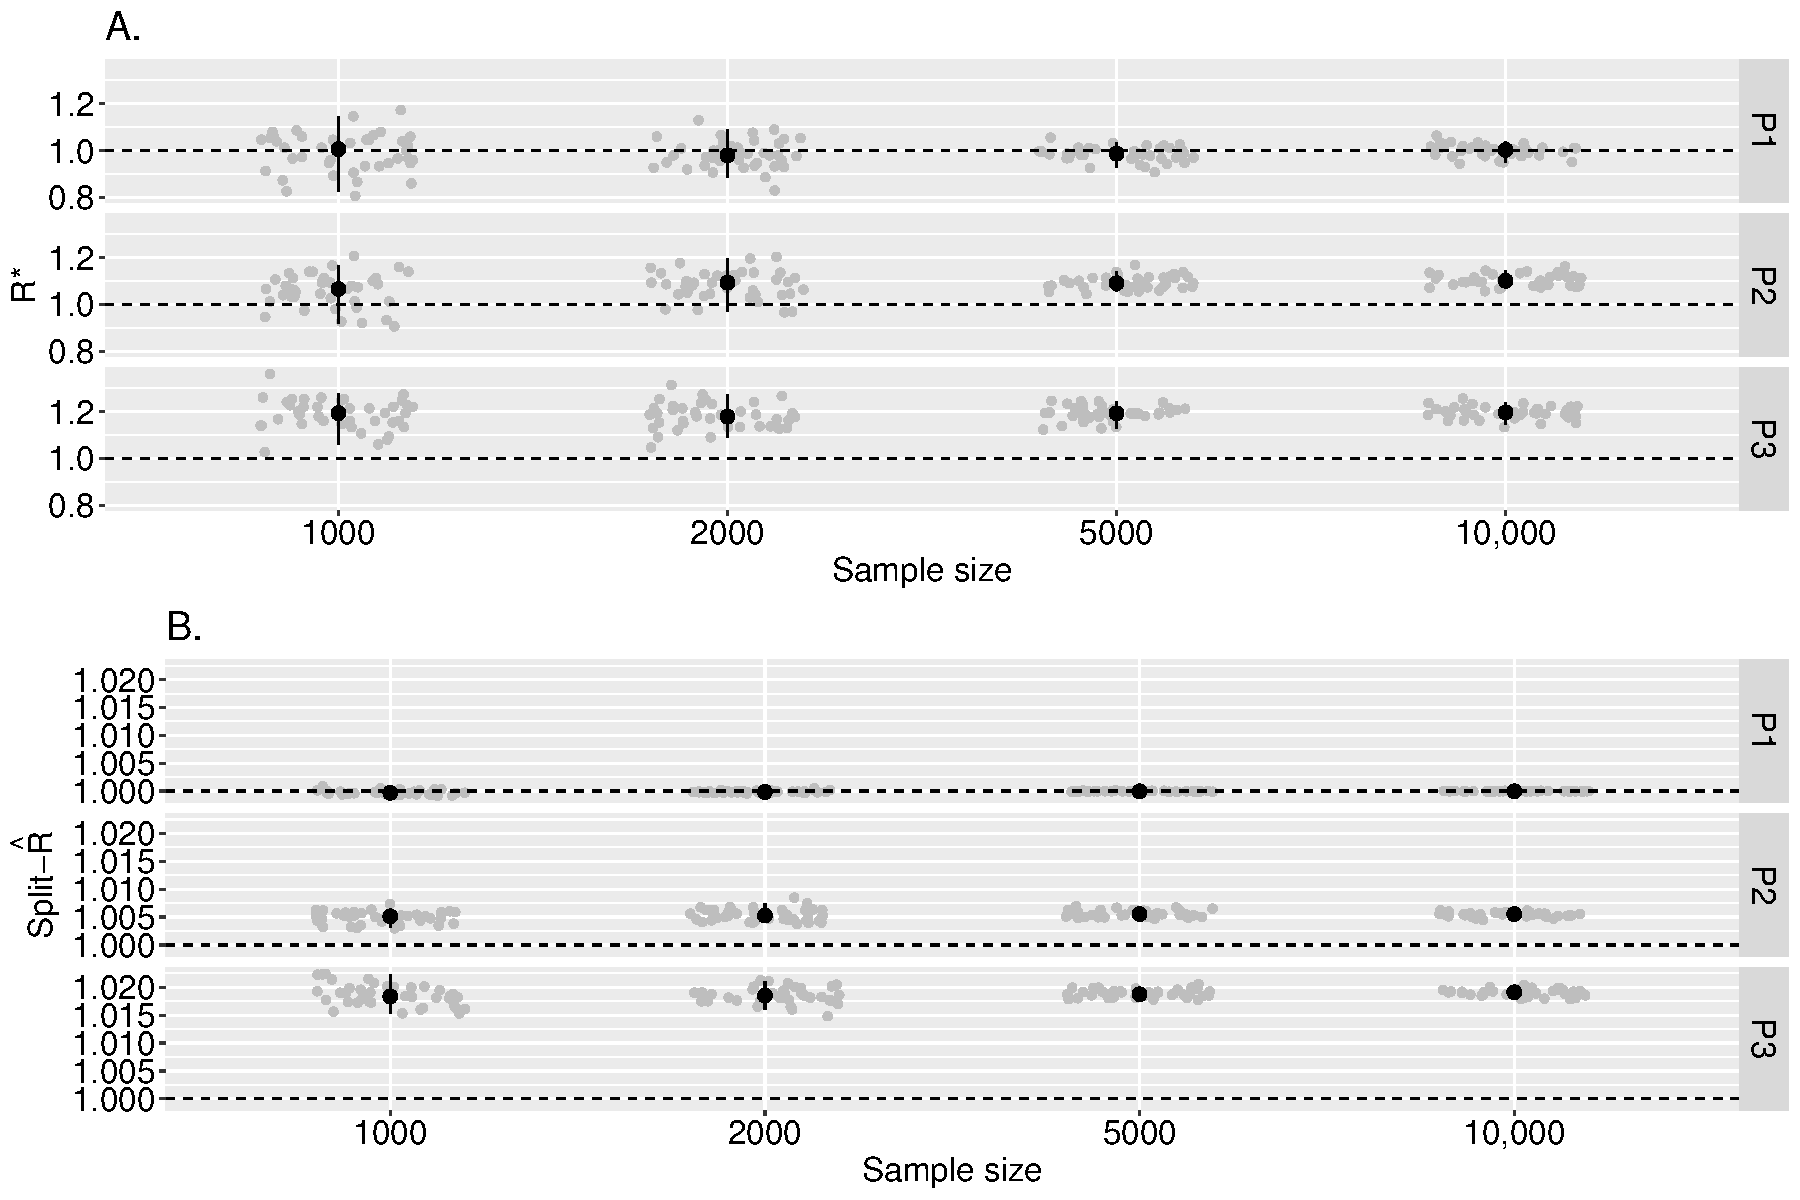
\includegraphics[width=1.0\textwidth]{discrete.pdf}}
	\caption{\textbf{Discrete distribution example: convergence diagnostics.} On the horizontal axis, we show the sample size of each set of simulations. The panels within A. and B. indicate the transition probability matrix used for the fourth chain (the other three chains always used $\boldsymbol{P}=\boldsymbol{P}_1$). In panel A, grey points indicate $R^*$ from each replicate calculated using Algorithm \ref{alg:R_star}) , and the black point-ranges indicate 2.5\% , 50\% and 97.5\% quantiles across the 40 replicates. In panel B, we show the same, but for split-$\widehat{R}$. The dashed horizontal lines at 1 indicate the convergence threshold in both cases.}
	\label{fig:discrete}
\end{figure}


\subsection{Large state-space}\label{sec:discrete_large}
We next consider a larger discrete parameter space: a univariate distribution with 20 states. As in \S\ref{sec:discrete_small}, we generate draws from three discrete Markov chains that share a common transition probability matrix, $\boldsymbol{P}$. For the fourth (and final) chain, we consider two cases: one where it shares the same matrix, $\boldsymbol{P}_1=\boldsymbol{P}$; the other, when its Markov process has a different matrix, $\boldsymbol{P}_2$. Rather than write down a given $\boldsymbol{P}$ and $\boldsymbol{P}_2$, we generated these stochastically: for each of the rows, we randomly sampled from from a Dirichlet process with shape vectors consisting of ones (of length 20).

To illustrate the differences between the two transition probability matrices, $\boldsymbol{P}$ and $\boldsymbol{P}_2$, we simulate 100,000 draws from each Markov process. In Fig. \ref{fig:discrete_stationary_higherd}, we show the marginal distribution obtained across all four chains: where the first three used $\boldsymbol{P}$, and the last used $\boldsymbol{P}_2$. In this plot, we show only the first four states of the 20-state model. The differences in marginal distributions between the first three chains and the last indicate that there are substantial differences in the target distributions.

\begin{figure}[!htb]
	\centerline{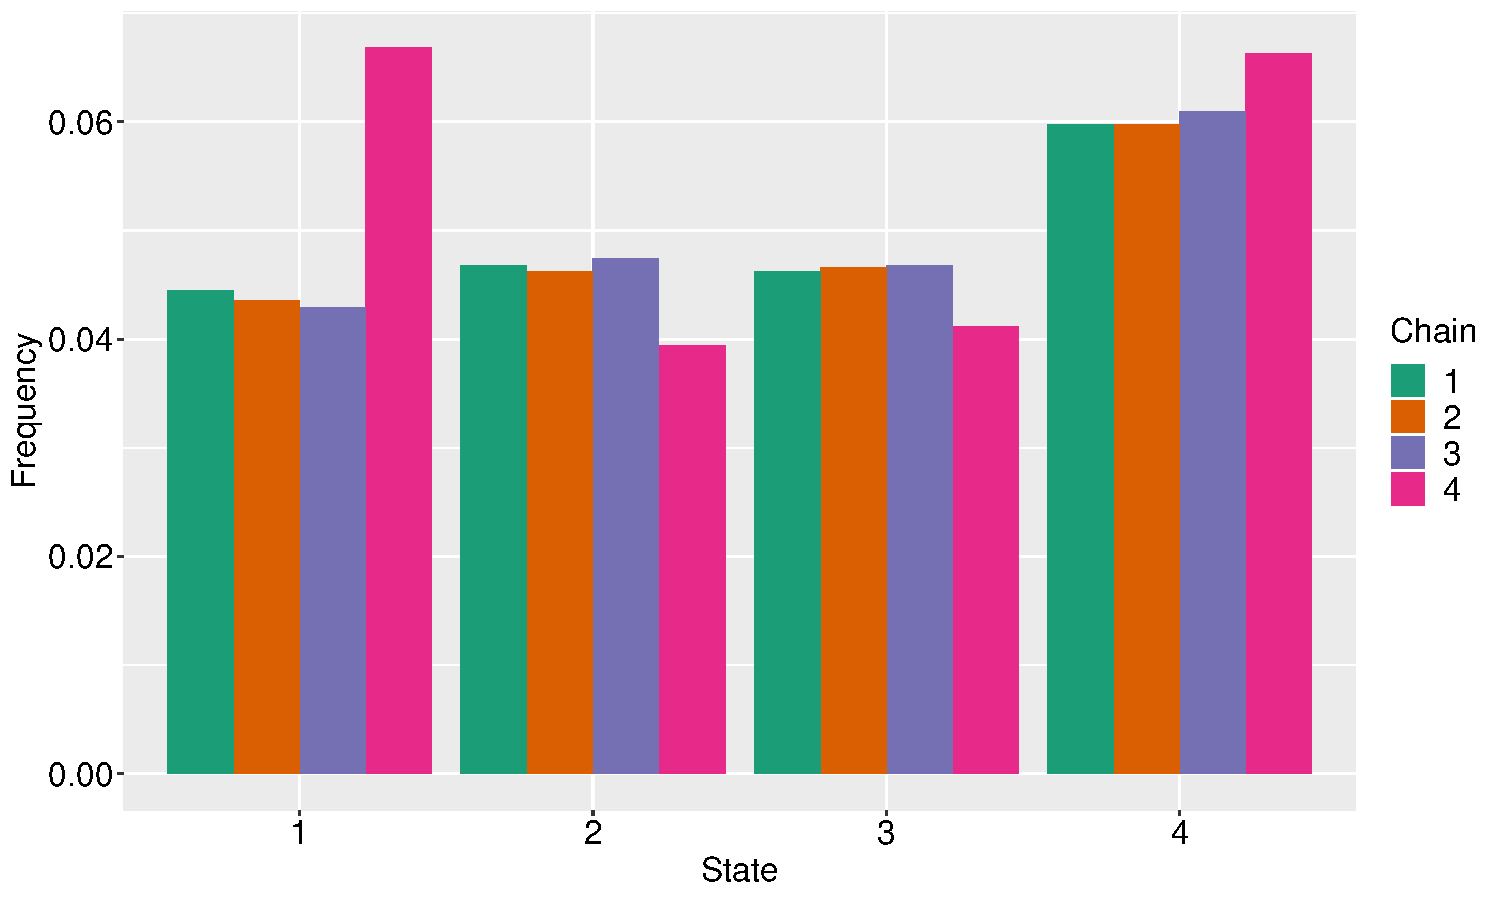
\includegraphics[width=1.0\textwidth]{discrete_stationary_higherd.pdf}}
	\caption{\textbf{Large state-space discrete distribution example: approximate stationary distribution.} The distribution over the first four states of a 20-state discrete model achieved after drawing 100,000 samples from each of four Markov chains. Here, the first three chains shared the same transition probability matrix; the last chain used a different matrix.}
	\label{fig:discrete_stationary_higherd}
\end{figure}

To probe the ability of $R^*$ and $\widehat{R}$ to detect poor convergence, we repeat the same exercise as in \S\ref{sec:discrete_small} although, here, we consider the new $\boldsymbol{P}_1$ and $\boldsymbol{P}_2$ cases. In Fig. \ref{fig:discrete_higherd}, we show the results of this analysis. This shows that $R^*\sim 1$ for the $\boldsymbol{P}_1$ case, correctly indicating no convergence issues; for the $\boldsymbol{P}_2$ case, $R^*>1$ across all replicates at sample sizes of 5000 and above. By contrast, $\widehat{R}$ struggles to differentiate between the $\boldsymbol{P}_1$ and $\boldsymbol{P}_2$ cases: in both instances, it signifies convergence.

\begin{figure}[!htb]
	\centerline{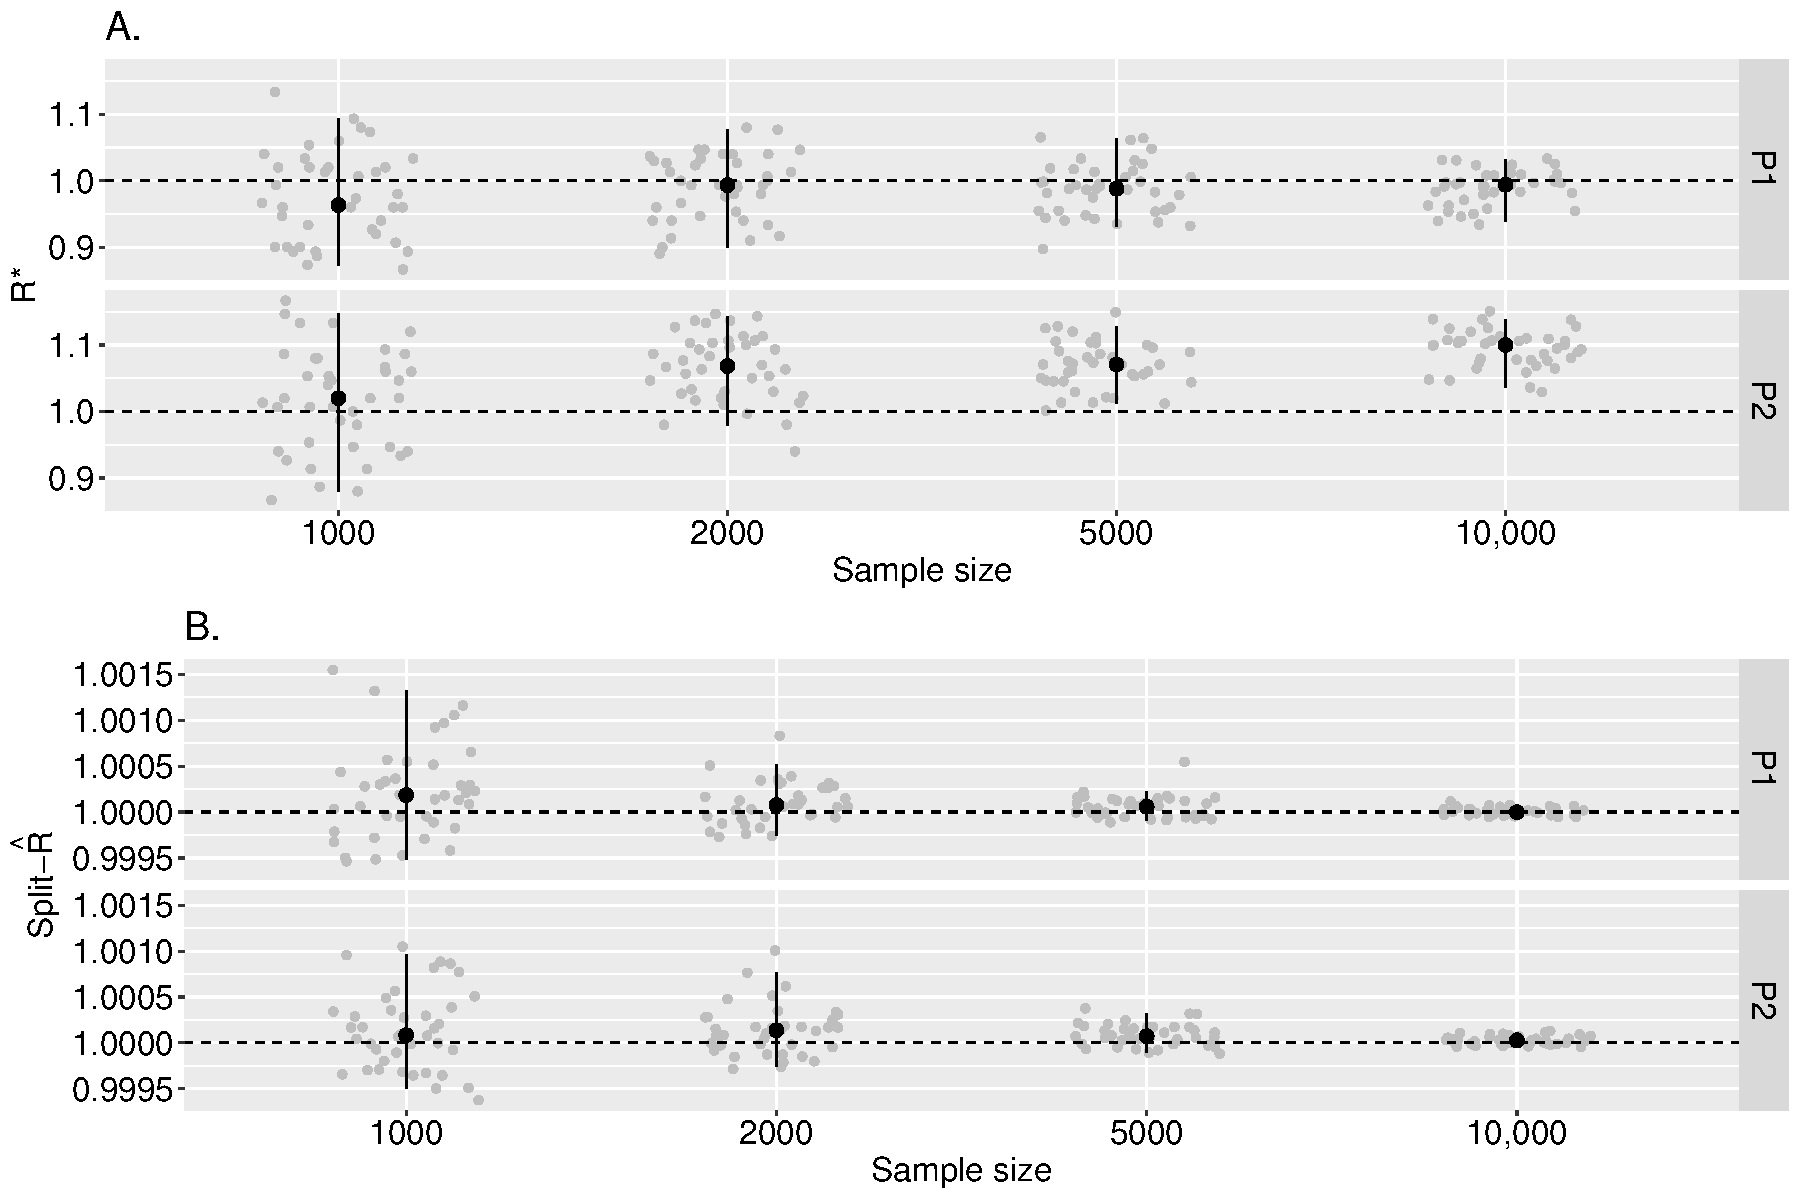
\includegraphics[width=1.0\textwidth]{discrete_higherd.pdf}}
	\caption{\textbf{Large state-space discrete distribution example: convergence diagnostics.} On the horizontal axis, we show the sample size of each set of simulations. The panels within A. and B. indicate the transition probability matrix used for the fourth chain (the other three chains always used $\boldsymbol{P}=\boldsymbol{P}_1$). In panel A, grey points indicate $R^*$ from each replicate calculated using Algorithm \ref{alg:R_star}) , and the black point-ranges indicate 2.5\% , 50\% and 97.5\% quantiles across the 40 replicates. In panel B, we show the same, but for split-$\widehat{R}$. The dashed horizontal lines at 1 indicate the convergence threshold in both cases.}
	\label{fig:discrete_higherd}
\end{figure}

Collectively, the results of \S\ref{sec:discrete_small} and \S\ref{sec:discrete_large} show that $R^*$ is able to detect convergence issues in discrete target distributions. The results of \S\ref{sec:discrete_large} hint that $R^*$ may be superior than $\widehat{R}$ in larger discrete spaces, although further empirical investigation is needed.

\color{black}

\color{red}
\section{ML sensitivity}\label{sec:ML_sensitivity}
In this section, we investigate how two decisions about classifiers — which classifier to use (in \S\ref{sec:ml_model}) and what hyperparameters to use for it (in \S\ref{sec:hyperparameters}) — affect calculation of $R^*$. The test cases used for empirical evaluation were selected from our pool of examples introduced in the text. Specifically, they were chosen to represent cases where $R^*$ was nearer 1, since, for these, small changes in calculated $R^*$ could lead to different decisions about convergence being reached. The four examples we used were:

\begin{itemize}
	\item The AR(1) example described in \S\ref{sec:heterogeneity}, except using 1000 draws per chain.
	\item The 250-dimensional non-centered multivariate normal example introduced in \S\ref{sec:multivariate_normal_250}. In each replicate, we generated 500 post-warm-up draws from the posterior (using 500 warm-up steps) using Stan's NUTS algorithm across each of 4 chains.
	\item The alternative parameterisation of the Cauchy model described in \S\ref{sec:cauchy}. For each replicate, we generated samples from the model using Stan's NUTS algorithm with 1000 post-warm-up draws (and 1000 warm-up draws) across each of 4 chains.
	\item The non-centered parameterisation of the eight schools model described in \S\ref{sec:eight_shools}. In each replicate, we used Stan's NUTS algorithm with adapt delta set to 0.95 to generate 1000 post-warm-up draws (and 1000 warm-up draws) across each of 4 chains; these were then used to calculate $R^*$.
\end{itemize}

\subsection{ML classifier comparison}\label{sec:ml_model}
In this section, we investigate how classification accuracy depends on choice of ML classifier. We restricted our analysis to popular classifiers with relatively few hyperparameters to simplify comparison amongst them. Notably, we do not consider neural network models, since the structure of nets effectively defines a high dimensional hyperparameter space.

The ML classifiers we compared were GBMs, RFs, k-nearest neighbours (KNNs), SVMs with linear kernels and a generalised linear model approach (GLM). All these models were called through the \textbf{\textsf{R}}'s Caret package \citep{kuhn2008building}: the GBM is implemented using the \textit{gbm} model in Caret which uses the ``gbm'' package \citep{greenwell2019package}; RFs are implemented using the \textit{rf} model in Caret which uses the ``randomForest'' \citep{liaw2002classification} package; KNN is natively implemented in Caret and called using the \textit{knn} model; SVMs are implemented in Caret using the \textit{svmLinear} model which uses ``kernlab'' package \citep{karatzoglou2004kernlab}; and the GLM is implemented through the \textit{multinom} model in the ``nnet'' package \citep{ripley2016package}.

Each of these classifiers has hyperparameters, and, due to the differences between the examples we consider (defined in \S\ref{sec:ML_sensitivity}), the optimal hyperparameters were likely to differ between examples. For each classifier-example combination, we first performed a single replicate of each experiment and choose those hyperparameters which maximised classification accuracy. The set of all hyperparameters we selected between were chosen so that training time for each classifier remained reasonable. These sets were the same across all examples:

\begin{itemize}
	\item GBM: Cartesian product of $\text{int.depth}=(3, 7)$; $\text{\# trees} = (50, 100)$;
	\item RF: $m_{\text{try}} = (1, 2)$. (Note, in \S\ref{sec:hyperparameters}, we investigate a dimension-specific approach to $m_{\text{try}}$ but, here, for ease of comparison with the other methods, we keep this static.)
	\item KNN: $K=(5,10,15, 20,40)$;
	\item SVM: $C=(0.25, 0.5, 0.75)$;
	\item GLM: $\text{decay}=(0.1, 0.2, 0.5, 1)$.
\end{itemize}

These hyperparameters were then used in subsequent replicates. We also used a different number of replicates at each unique combination of classifier and hyperparameters across the experiments due to the differing demands of each example: for the AR(1) example, we used 100 replicates; for the multivariate normal example, we used 100; for the Cauchy model, 50 replicates; and for the eight schools model, 30 replicates.

The results of these experiments are shown in Fig. \ref{fig:ml_comparison_all}. The top row shows $R^*$ as calculated by each classifier (in each case, chains split into two halves); the bottom row shows the time (in seconds) taken for $R^*$ calculation. The panels correspond to the examples described in \S\ref{sec:ML_sensitivity}. Across the examples, the classification accuracy of RFs and GBMs were, generally, highest; followed by KNNs. An exception was for the 250-dimensional normal where KNN performed best. In the AR(1) example, GBM outperformed RF. In higher dimensional cases, RF outperformed GBM. In all cases, RF and GBM classifiers took the greatest time to train; in higher dimensional examples, RF-based $R^*$ were cheaper to calculate than those from GBMs.


\begin{figure}[!htb]
	\centerline{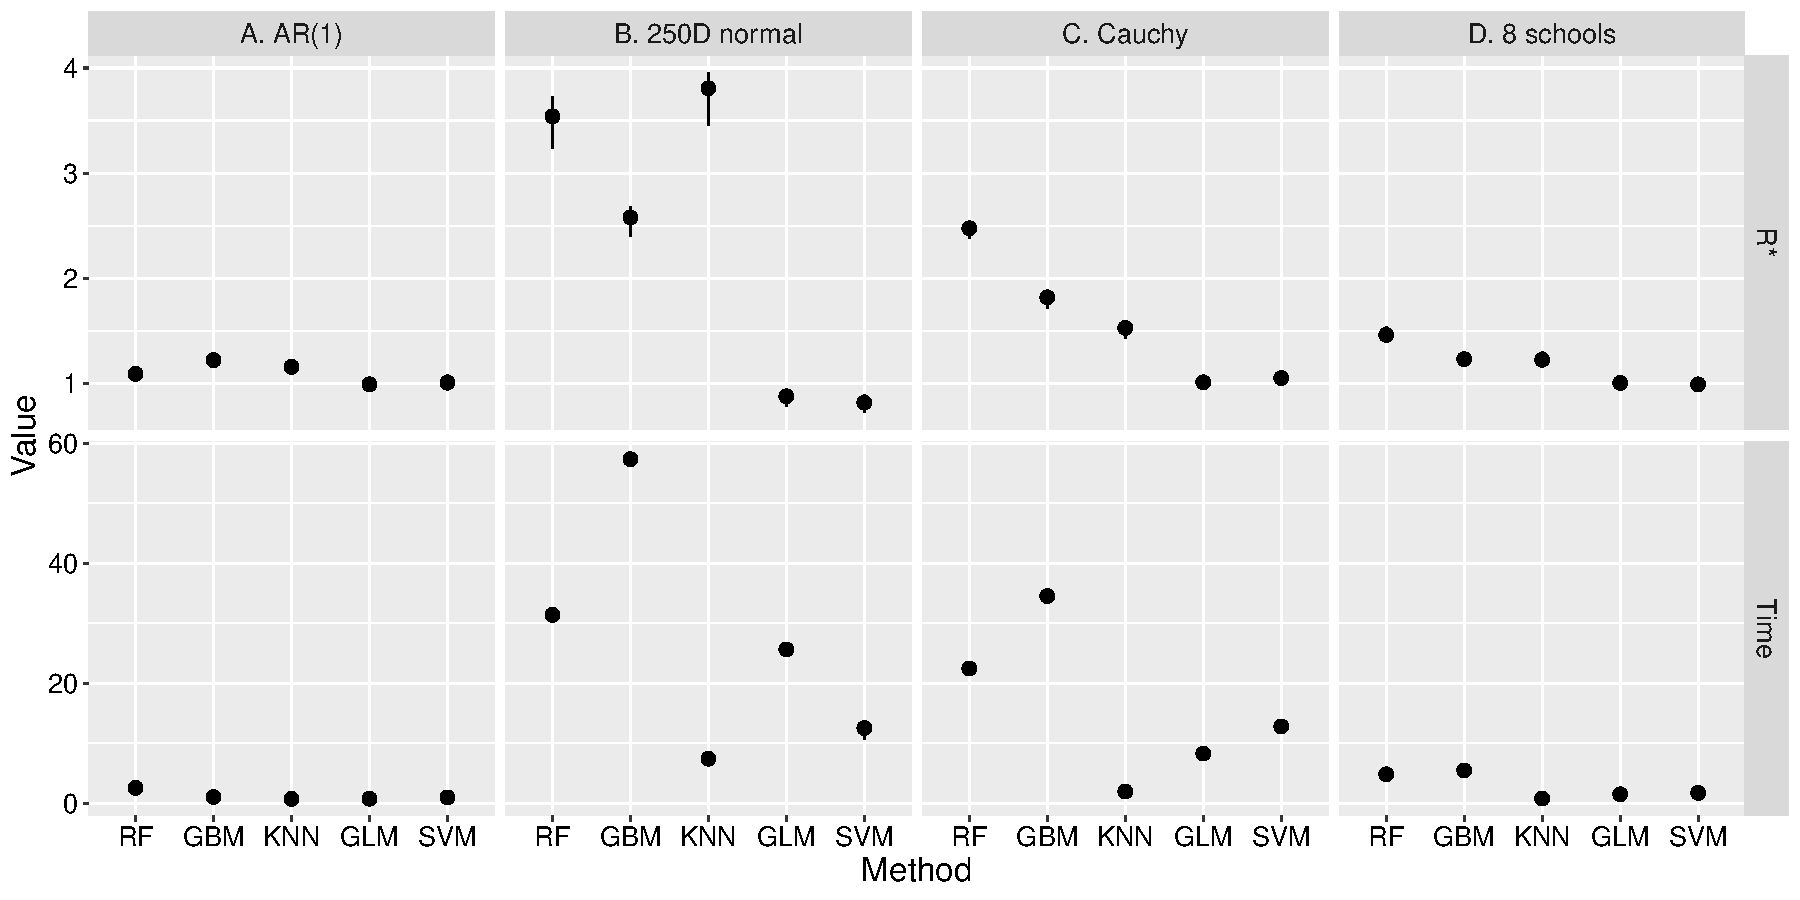
\includegraphics[width=1.0\textwidth]{ml_comparison_all.pdf}}
	\caption{\textbf{ML classifier comparison.} Top row shows $R^*$ values calculated using Algorithm \ref{alg:R_star}; bottom row show the time taken to run each method on a desktop computer. The different columns correspond to the examples described in \S\ref{sec:ML_sensitivity}. Black point-ranges indicate 25\% , 50\% and 75\% quantiles across all replicates; note, that the number of replicates varies across examples as given in \S\ref{sec:ml_model}.}
	\label{fig:ml_comparison_all}
\end{figure}

\color{black}

\color{red}
\subsection{Hyperparameter sensitivity}\label{sec:hyperparameters}
In this section, we considered only the two classifiers — GBMs and RFs — that performed best on our comparison between ML methods in \S\ref{sec:ml_model}. The performance of GBMs and RFs, like most ML methods, depends on their hyperparameters. In GBMs, a regression function is approximated by additive components, where each of those corresponds to a tree. The number of such regression trees is thus a hyperparameter of the model. Each regression tree can split amongst any integer number of variables (the \textit{interaction depth}). For GBMs, we analyse how their performance depends on these two hyperparameters. For RFs, there is a single hyperpameter: $m_{\text{try}}$, the number of members of the subset of all features over which to search for an optimal split when forming a decision tree. Note, that the maximum allowed value of $m_{\text{try}}=K$ — the dimensionality of the target distribution. 

In this section, we investigate the sensitivity of $R^*$ calculated by GBMs and RFs to each of these sets of hyperparameters across a range of examples (defined in \S\ref{sec:ML_sensitivity}). Since each example is of different dimensionalities, we compare different sets of hyperparameters in each, although include amongst the sets the default values we suggest for each classifier in \S\ref{sec:method} (these are shown as triangles on the plots). Note, that for the GBM model, we did not investigate a full range of hyperparameters needed to optimise $R^*$ for many of the examples due to the extensive training time needed to do so. For RFs, runtime was less restrictive and we were better able to survey the sensitivity across hyperparameter space.

We also used a different number of replicates at each unique combination of classifier and hyperparameters across the experiments due to the differing demands of each example: for the AR(1) example, we used 200 replicates; for the multivariate normal example, we used 20; for the Cauchy model, 20 replicates; and for the eight schools model, 50 replicates.


\subsubsection{Autoregressive example}\label{sec:hyperparameters_ar1}
In Fig. \ref{fig:hypers_ar1}, we show the results of the AR(1) analysis. In panel A, we show the sensitivity of $R^*$ as calculated by GBMs to variation in hyperparameters. In panel B, we show the same but for RFs. In both panels, the results for the parameterisation we suggest as defaults is shown as a triangle. For the GBM model, $R^*$ varied according to hyperparameters: of the set investigated, an interaction depth of 1 appears optimal with 10+ trees. In panel B, the values of $R^*$ are generally lower than those achieved by GBMs. As shown in \S\ref{sec:comparison_gbm_rf}, RFs appear less well-suited to lower dimensional problems. Across the two possible hyperparameter values for RFs, there was not a substantial difference in the values of $R^*$ calculated.

\begin{figure}[!htb]
	\centerline{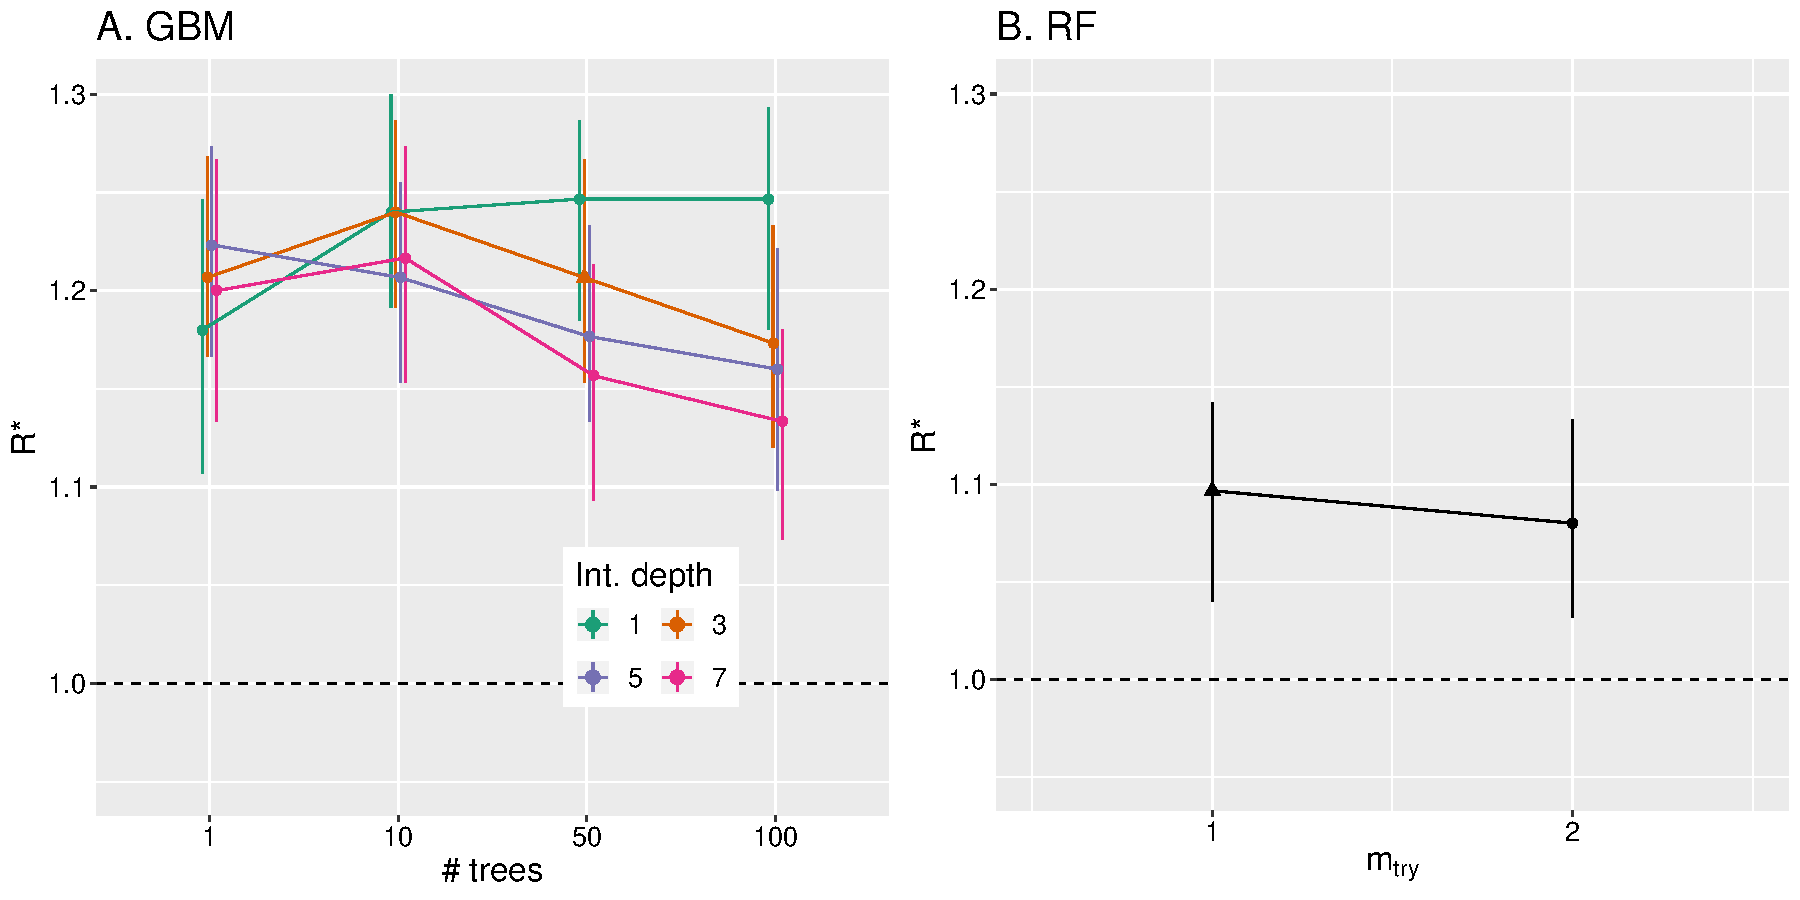
\includegraphics[width=1.0\textwidth]{hypers_ar1.pdf}}
	\caption{\textbf{Hyperparameter sensitivity: AR(1) example.} Panel A shows the sensitivity of GBM-derived $R^*$ to hyperparameter variation for the AR(1) example described in \S\ref{sec:hyperparameters_ar1}; Panel B shows the same but for a RF classifier. Black point-ranges indicate 25\% , 50\% and 75\% quantiles across all replicates. In Panel A, the coloured lines shows the different interaction depths investigated. In both panels, the results for the parameterisation we suggest as defaults is shown as a triangle.}
	\label{fig:hypers_ar1}
\end{figure}

\subsubsection{Multivariate normal: 250-dimensional model}\label{sec:hyperparameters_normal}
In Fig. \ref{fig:hypers_normal}, we show the results of the analysis for the 250-dimensional normal example. In panel A, we show the sensitivity of $R^*$ as calculated by GBMs to variation in hyperparameters. In panel B, we show the same but for RFs. This shows that $R^*$ was higher as calculated by RFs and that performance of GBMs depended strongly on hyperparameters.

\begin{figure}[!htb]
	\centerline{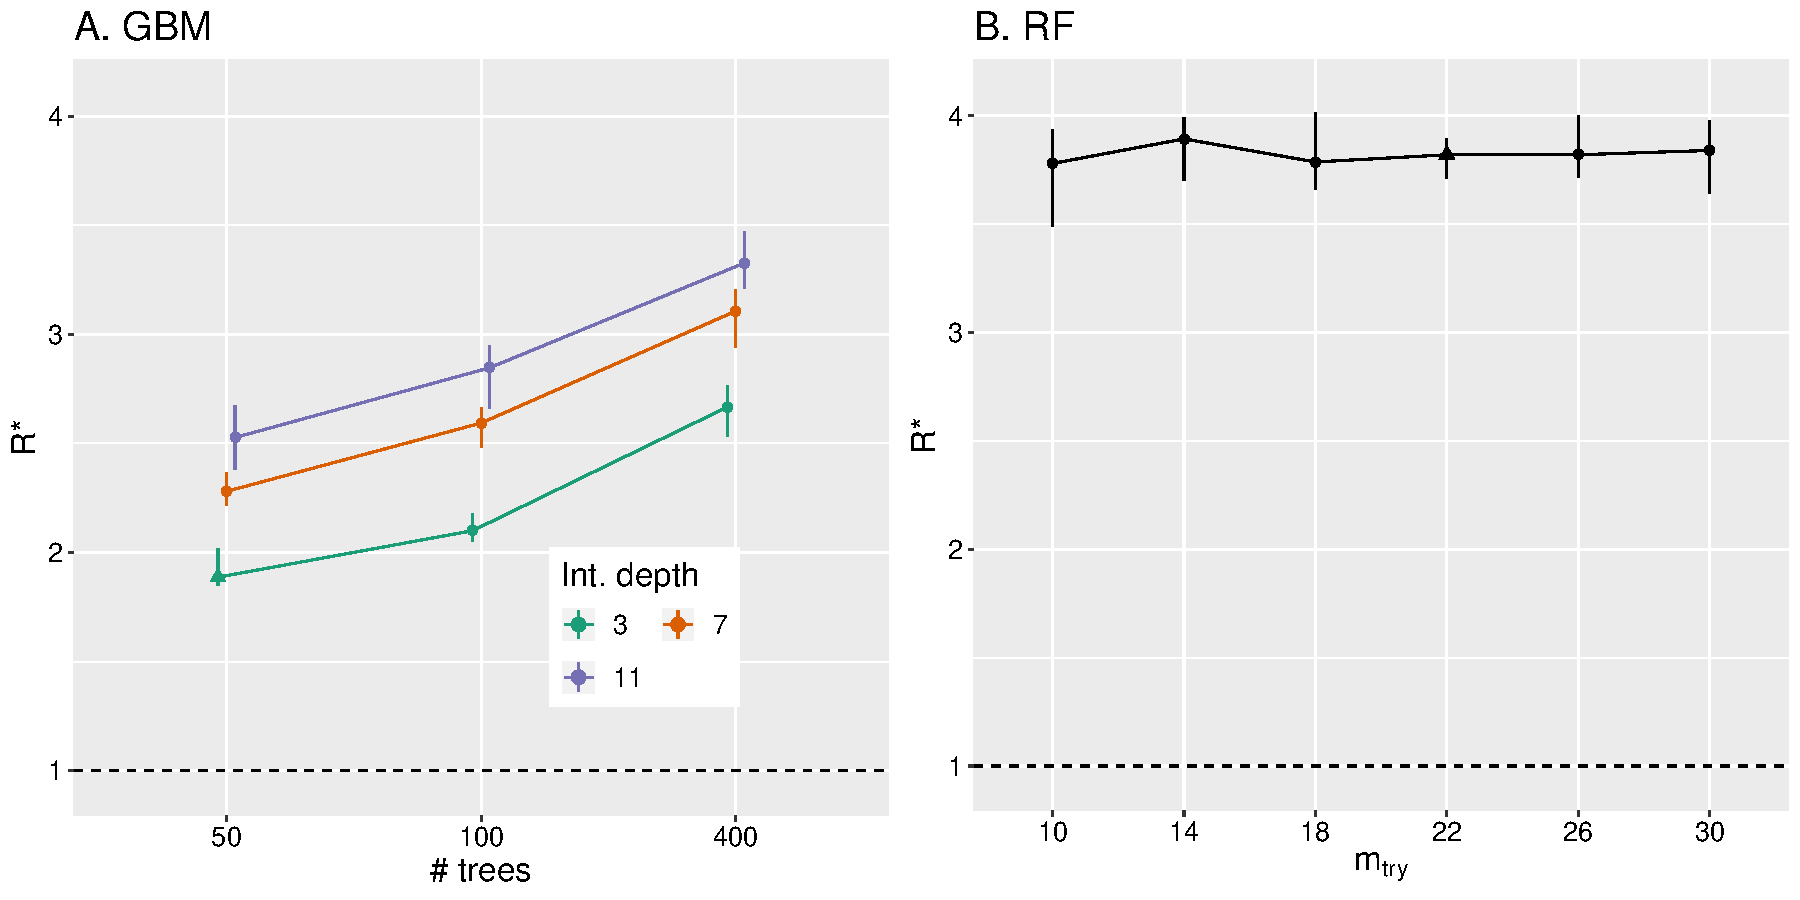
\includegraphics[width=1.0\textwidth]{hypers_normal_250.pdf}}
	\caption{\textbf{Hyperparameter sensitivity: 250-dimensional normal example.} Panel A shows the sensitivity of GBM-derived $R^*$ to hyperparameter variation for the Cauchy example described in \S\ref{sec:hyperparameters_normal}; Panel B shows the same but for a RF classifier. Black point-ranges indicate 25\% , 50\% and 75\% quantiles across all replicates. In Panel A, the coloured lines shows the different interaction depths investigated. In both panels, the results for the parameterisation we suggest as defaults is shown as a triangle.}
	\label{fig:hypers_normal}
\end{figure}


\subsubsection{Cauchy model: alternative parameterisation}\label{sec:hyperparameters_cauchy}
In Fig. \ref{fig:hypers_cauchy}, we show the results of the Cauchy model analysis. In panel A, we show $R^*$ as calculated by a GBM classifier; in panel B, the same but using a RF classifier. In both panels, the results for the parameterisation we suggest as defaults is shown as a triangle. Across the range of hyperparameters investigated, the RF classifier outperformed the GBM and was less sensitive to variation in its hyperparameters.

\begin{figure}[!htb]
	\centerline{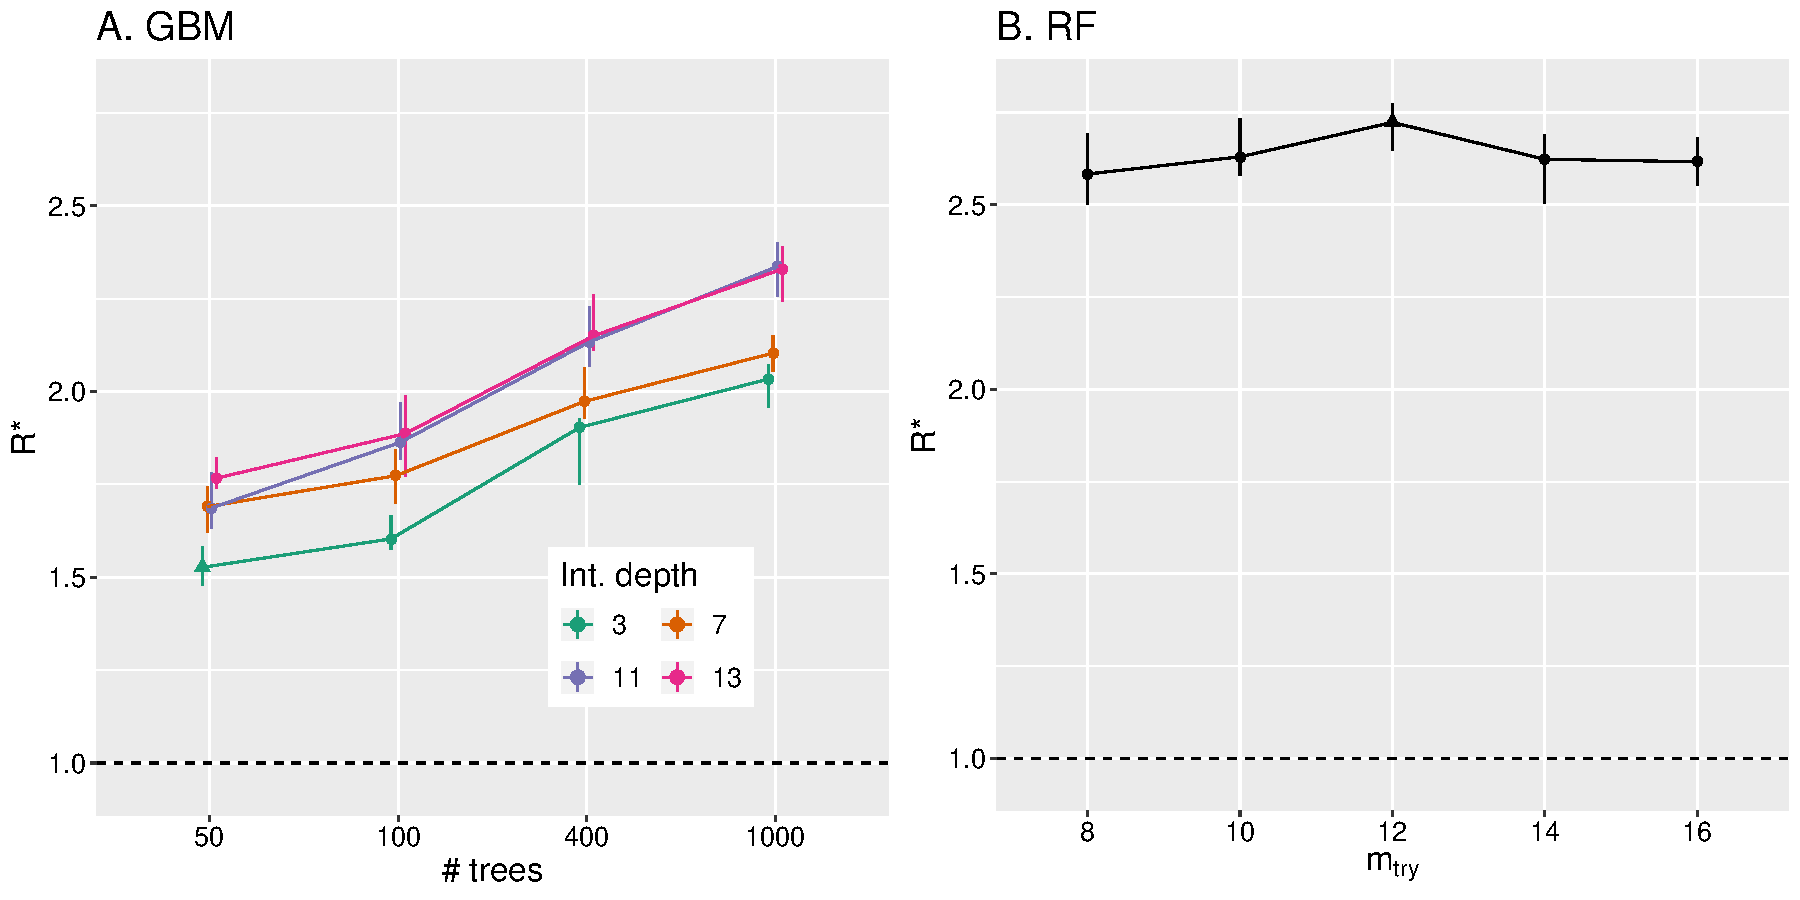
\includegraphics[width=1.0\textwidth]{hypers_cauchy.pdf}}
	\caption{\textbf{Hyperparameter sensitivity: Cauchy example.} Panel A shows the sensitivity of GBM-derived $R^*$ to hyperparameter variation for the Cauchy example described in \S\ref{sec:hyperparameters_cauchy}; Panel B shows the same but for a RF classifier. Black point-ranges indicate 25\% , 50\% and 75\% quantiles across all replicates. In Panel A, the coloured lines shows the different interaction depths investigated. In both panels, the results for the parameterisation we suggest as defaults is shown as a triangle.}
	\label{fig:hypers_cauchy}
\end{figure}

\subsubsection{Eight schools: non-centered parameterisation}\label{sec:hyperparameters_8_schools}
In Fig. \ref{fig:hypers_8_schools}, we show the results of the experiments on the eight schools model. Panel A shows how $R^*$ calculated using a GBM varies with its two hyperparameters; panel B shows the same but for RFs. This shows that, in this case, the value of $R^*$ calculated by RFs was higher than that for GBMs. Further, whereas GBMs were relatively sensitive to their hyperparameter values, RFs were less so.

\begin{figure}[!htb]
	\centerline{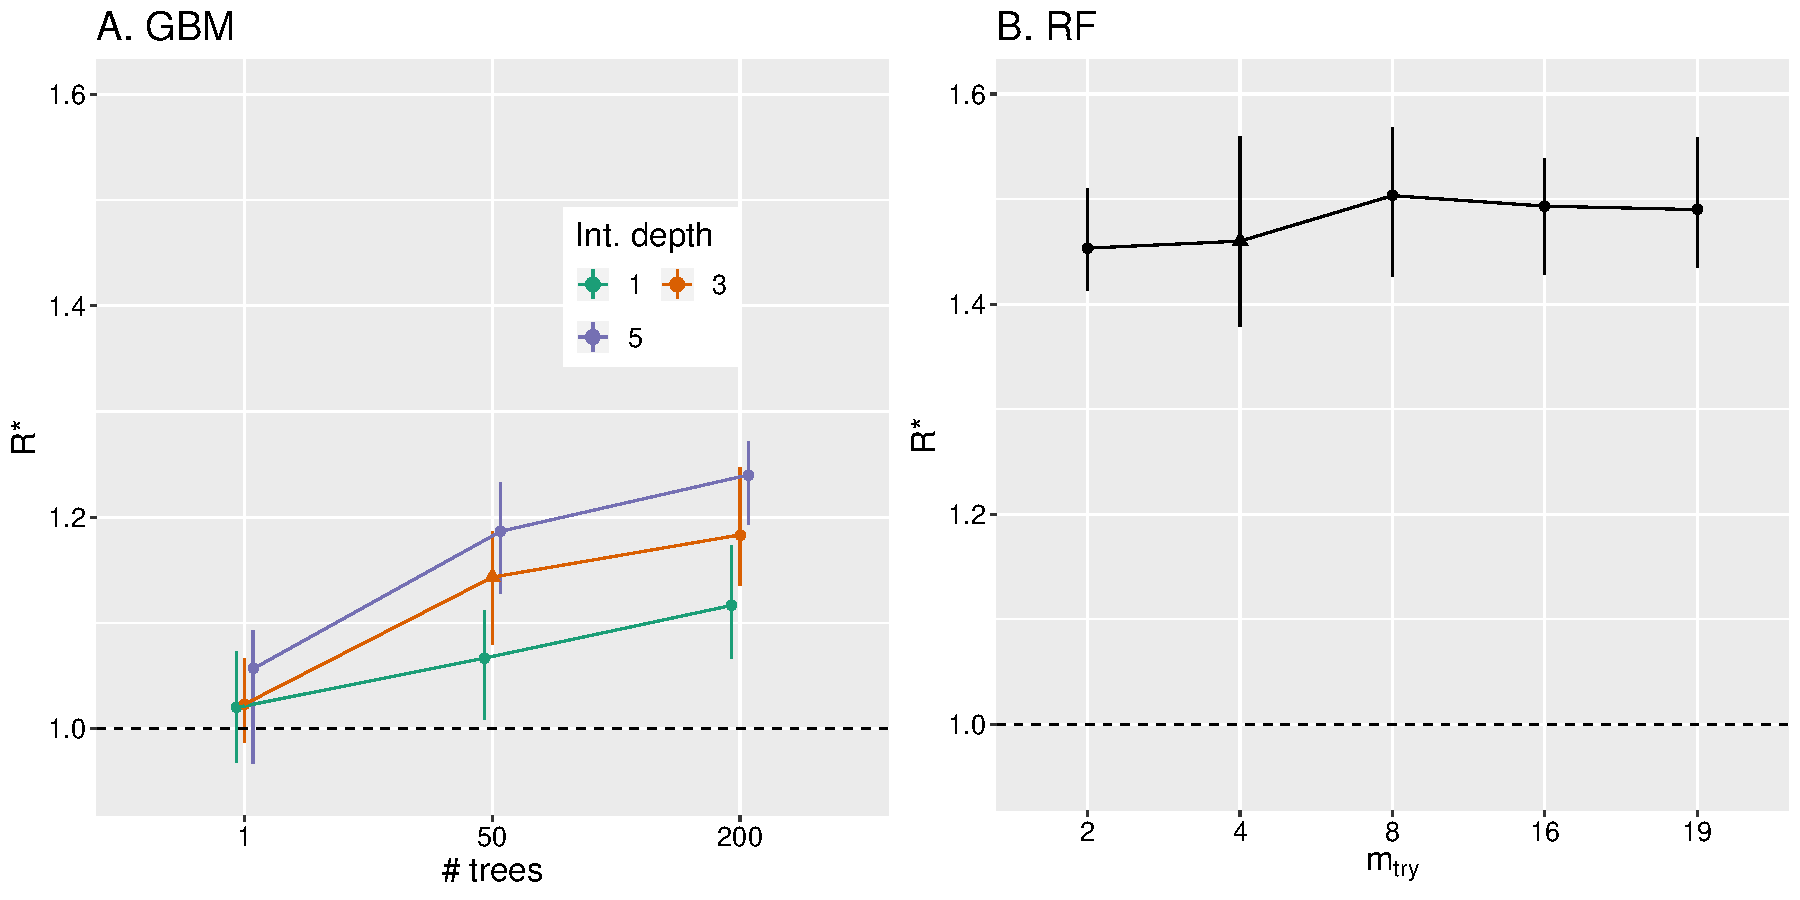
\includegraphics[width=1.0\textwidth]{hypers_8_schools.pdf}}
	\caption{\textbf{Hyperparameter sensitivity: eight schools example.} Panel A shows the sensitivity of GBM-derived $R^*$ to hyperparameter variation for the eight schools example described in \S\ref{sec:hyperparameters_8_schools}; Panel B shows the same but for a RF classifier. Black point-ranges indicate 25\% , 50\% and 75\% quantiles across all replicates. In Panel A, the coloured lines shows the different interaction depths investigated. In both panels, the results for the parameterisation we suggest as defaults is shown as a triangle.}
	\label{fig:hypers_8_schools}
\end{figure}

\color{black}

\color{red}
\section{Comparing GBMs and RFs}\label{sec:comparison_gbm_rf}
In \S\ref{sec:ML_sensitivity}, we present a series of experiments using popular ML methods and find that, among these methods, GBMs and RFs perform most consistently across them. In this section, we compare $R^*$ derived from using a GBM classifier with that from a RF classifier. In these experiments, we fix the hyperparameters of each as given in \S\ref{sec:method}. In \S\ref{sec:joint_distribution}, we compare how both methods are able to diagnose lack of convergence in a joint distribution. In \S\ref{sec:tail_fatness}, we compare the ability of both approaches to diagnose differences in the tails of the marginal distributions between chains. Since we use independent sampling to generate draws, we are also able to calculate the \textit{Bayes optimal} classification accuracy, which is the classifier that minimises the probability of misclassification error \citep{devroye2013probabilistic}. This classifier assigns chain identities according to the one which has the maximum posterior probability of having generated a draw. Here, we assume that \textit{a priori} all chains are equally likely to have generated the data, so the classifier categorises draws to the chain which maximises the likelihood of that observation.

\subsection{Joint distribution}\label{sec:joint_distribution}
Here, we consider a multivariate normal target distribution with dimensionality ranging from 1 to 32. For three `chains', we generated 2000 draws by independently sampling from a multivariate normal with zero mean and given covariance matrix; for the fourth chain, the same number of draws are generated in the same way except with a different covariance matrix. To generate the covariance matrices, we randomly sampled two 32-dimensional covariance matrices from the LKJ distribution with degrees of freedom 1 \citep{lewandowski2009generating}: note, that this results in matrices with unit diagonal values, meaning the marginal distributions of each dimension are standard normals. To obtain covariance matrices for the targets with dimensions, $d<32$, submatrices, $A^{\{d\}}$, were constructed from the 32-dimensional covariance matrices by taking leading blocks from them: $A^{\{d\}}:=A^{\{32\}}_{1:d, 1:d}$. For each target, we performed 20 replicates, where in each case, $R^*$ was calculated using GBM and RF classifiers. In addition, we determined an $R^*$ using the Bayes optimal classifier: to do so, we generated 10,000 draws from the four-chain process and assign chain identities to the maximum likelihood class.  

The results of these experiments are shown in Fig. \ref{fig:gbm_vs_rf_normal}. In this plot, the bottom axis shows the dimensionality of the target distribution; the vertical axis shows $R^*$, and the point colour and shadings give the method used to calculate this statistic. When the target is unidimensional, the four chains have the same target distribution and the optimal $R^*=1$. In this case, both the GBM and RF methods produce classification rates that overlap with this value, indicating convergence. As the number of dimensions increases, it becomes easier to differentiate between samples from the two processes and the optimal $R^*$ grows. $R^*$ as calculated by GBMs and RFs also increases. For a two-dimensional target, the GBM method outperforms the RF one, getting closer to optimal classification. For higher dimensional targets, the RF classifier outperforms, achieving near-optimal $R^*$ in 32 dimensions.

\begin{figure}[!htb]
	\centerline{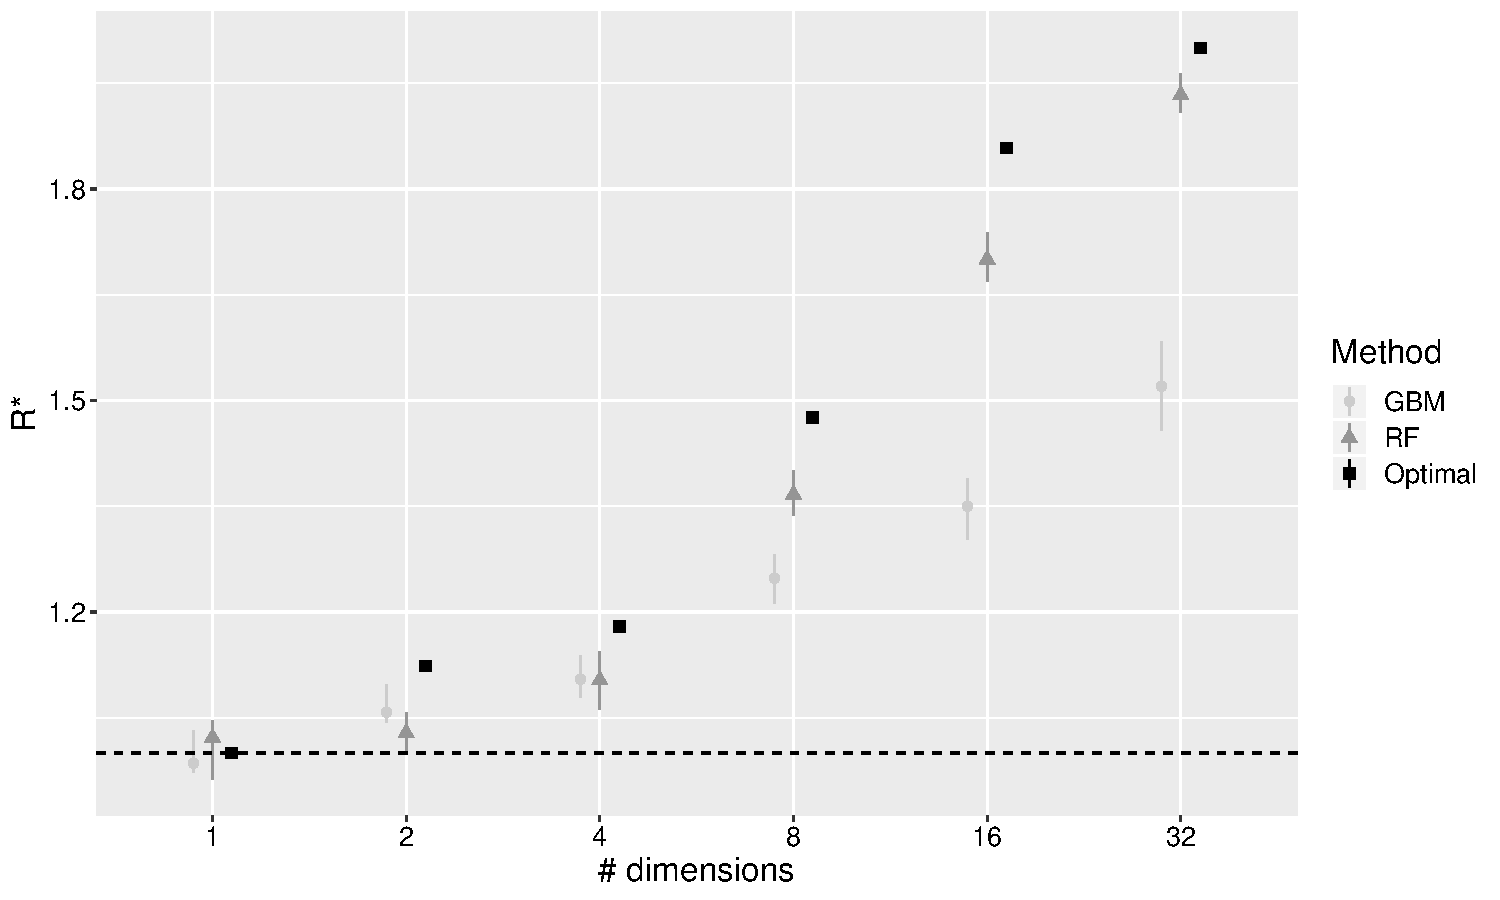
\includegraphics[width=1\textwidth]{gbm_vs_rf_normal.pdf}}
	\caption{\textbf{GBM versus RF: multivariate normal.} The horizontal axis gives the dimensions of the target distribution; the vertical axis gives the value of $R^*$ as calculated by Algorithm \ref{alg:R_star} using a GBM (light grey points), a RF (dark grey triangles) and the Bayes optimal classifier (black squares). The upper and lower point ranges show the 75\% and 25\% quantiles and the filled shapes show the medians. For the Bayes optimal classifier, there is only a point estimate since the optimal accuracy was estimated by Monte Carlo sampling using 10,000 draws from the four chain process. The dashed line shows $R^*=1$. Here, $R^*$ was calculated using chains split into two halves.}
	\label{fig:gbm_vs_rf_normal}
\end{figure}

\subsection{Fat tails}\label{sec:tail_fatness}
We now compare how the GBM and RF methods are able to diagnose lack of convergence in the tails of a target distribution. To do so, we again consider four chains. In three of these chains, we generated 2000 draws by randomly sampling from a multivariate Student-t distribution with mean zero and 3 degrees of freedom. In the remaining chain, we generated the same number of independent draws but use a mean-zero multivariate Student-t distribution with differing degrees of freedom, $\nu$. We consider a range of target dimensions: to generate the shape matrix for the first three chains, we use the same approach as in \S\ref{sec:joint_distribution} to build up appropriate shape matrices for each target dimensions, $A^{\{d\}}$. We examine a range of values of $\nu=\{4, 8, 16, 32\}$, representing decreasing tail fatness. Across the range of $\nu$ considered, the covariance matrix for the first three chains is given by $\nu/{(\nu-2)} A^{\{d\}}$. To ensure that the fourth chain has the same covariance as the first three, we use a shape matrix ${(\nu-2)}/\nu A^{\{d\}}$. For each combination of dimensions and $\nu$, we performed 20 replicates, where in each, we again calculate $R^*$ for both the GBM and RF classifiers. Additionally, we estimate an optimal $R^*$ using the Bayes optimal classifier by calculating the predictive accuracy of 10,000 draws of the four-chain process.

The results of these experiments are shown in Fig. \ref{fig:gbm_vs_rf_studdentt}. Here, each panel shows a target distribution of different dimensionality: 1, 2, 4, 8, 16 and 32 dimensions. Within each panel, the horizontal axis shows the degrees of freedom, $\nu$, of the fourth chain; the vertical axis gives $R^*$. The point colour and shadings give the method used to calculate $R^*$. In each panel, increases in $\nu$ make it easier to differentiate draws from the fourth chain from those of the first three: accordingly $R^*$ tends to increase for each method. As the target dimensionality increases (panels left-right along each row), it also becomes easier to contrast draws from the fourth chain, and $R^*$ increases. In all cases, the optimal $R^*$ exceeds those using GBM or RF classifiers. In 1-4 dimensions, the GBM approach outperforms the RF one, getting closer to the optimal classification rate. If the number of dimensions is 16 or greater, the order switches, and RFs often outperform GBMs.


\begin{figure}[!htb]
	\centerline{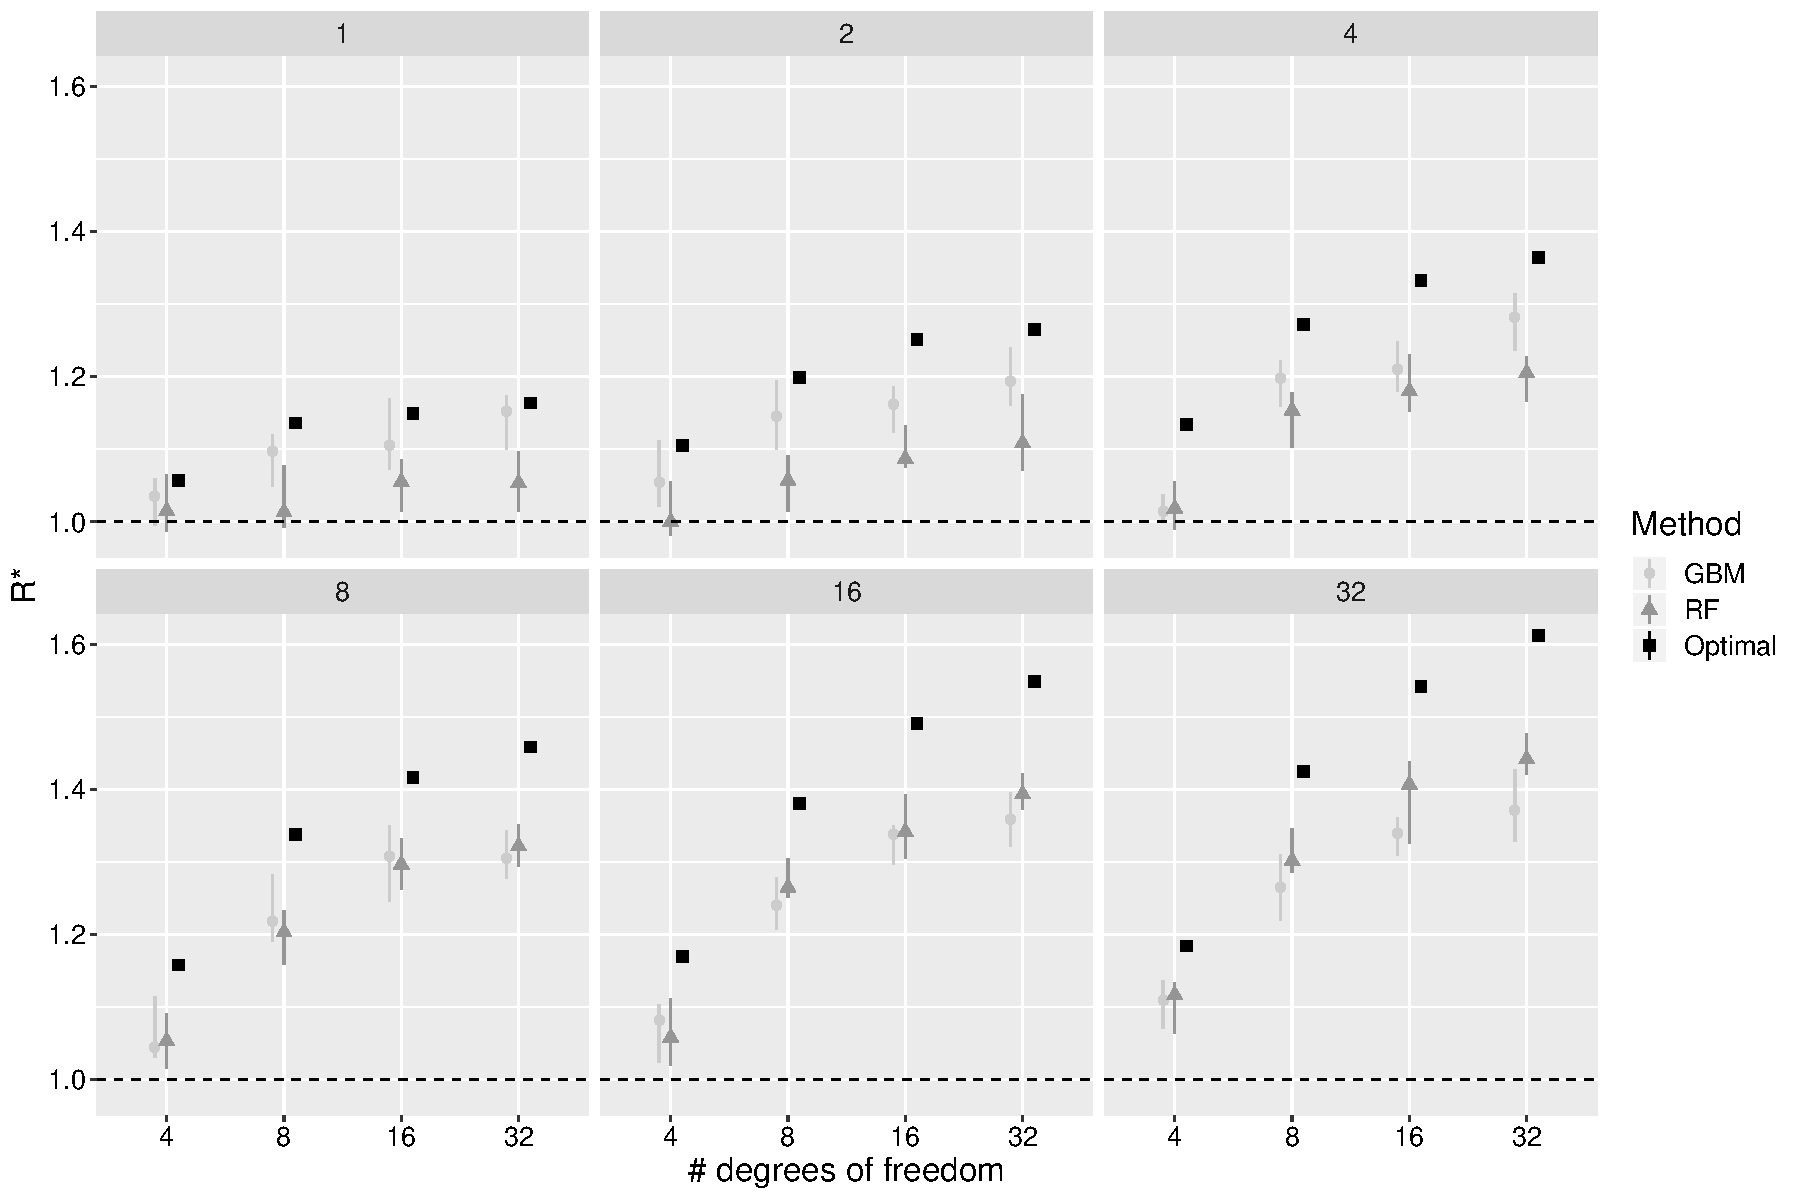
\includegraphics[width=1\textwidth]{gbm_vs_rf_studentt.pdf}}
	\caption{\textbf{GBM versus RF: multivariate Student-t.} Different panels show the various dimensions of the target distribution. The horizontal axis gives the degrees of freedom of the multivariate Student-t distribution for the fourth chain; the vertical axis gives the value of $R^*$ as calculated by Algorithm \ref{alg:R_star} using a GBM (light grey points), a RF (dark grey triangles) and the Bayes optimal classifier (black squares). The upper and lower point ranges show the 75\% and 25\% quantiles and the filled shapes show the medians. For the Bayes optimal classifier, there is only a point estimate since the optimal accuracy was estimated by Monte Carlo sampling using 10,000 draws from the four chain process. The dashed line shows $R^*=1$. Here, $R^*$ was calculated using chains split into two halves.}
	\label{fig:gbm_vs_rf_studdentt}
\end{figure}
\color{black}

\bibliographystyle{chicago}
\bibliography{bibliography} 

\end{document}